\documentclass[aspectratio=43]{beamer}
\useoutertheme[height=10mm,width=14mm,hideallsubsections]{sidebar}
\usetheme{PaloAlto}
\usecolortheme{clover}
\setbeamercovered{transparent}
\setbeamertemplate{navigation symbols}{}
\setbeamertemplate{sections in toc}{[ball unnumbered]}
\usepackage{times}
\usefonttheme{structurebold}
\usepackage[english]{babel}
\usepackage{amsmath,amssymb,amsfonts}
\usepackage{graphicx,color,multimedia,verbatim}
\usepackage[utf8]{inputenc}
\usepackage{listings}
\usepackage{hyperref}
\usepackage{tikz,tikzscale}

\def\dealrelease{9.1.1}
\lstset{escapechar=\%}

%\date[Software Frameworks]{Software Frameworks\\ for Challenging
%  Computational Problems\\Heraklion, January 14--18, 2013}
\date[IITK 2020]{Indian Institute of Technology Kanpur\\
  February 29 -- March 2nd, 2020}
%\date[PIMS 2016]{University of British Columbia\\ August 29 -- September 1st, 2016}
\title[deal.II Course]{Short Course on Partial differential equations with deal.II}
\author[Kanschat/Dond]{Guido Kanschat, Asha Kisan Dond}
\institute[IWR HD \& IISER TVM]{IWR, Universität Heidelberg
and IISER Thiruvananthapuram
  \\[2mm]
%  Department of Mathematics, Texas A\&M University\\[5mm]

\includegraphics[height=.13\textheight]{iwr}
\hfill

\includegraphics[height=.13\textheight]{dealclover}
\hfill

\includegraphics[height=.15\textheight]{unihd}
\hfill

\includegraphics[height=.15\textheight]{iiserlogo}
}
%
\pgfdeclareimage[height=10mm]{logo}{dealclover}
\logo{\pgfuseimage{logo}}
%
\def\R{\mathbb R}
\def\T{\mathbb T}                           % triangulation
\def\divh{\nabla_h\!\cdot}
\def\red{\color{red}}
\def\blue{\color{blue}}
\def\black{\color{black}}
\definecolor{green}{rgb}{0, .7, 0}
\def\green{\color{green}}
%
\input{only}
%
\hypersetup{urlcolor=blue}
\newcommand{\myurl}[2]{\underline{\href{#1}{#2}}}
\begin{document}
\begin{frame}[plain]
  \titlepage    
\end{frame}

%%%%%%%%%%%%%%%%%%%%%%%%%%%%%%%%%%%%%%%%%%%%%%%%%%%%%%%%%%%%%%%%%%%%%%
%%%%%%%%%%%%%%%%%%%%%%%%%%%%%%%%%%%%%%%%%%%%%%%%%%%%%%%%%%%%%%%%%%%%%%
\subsection*{Tutorial Structure}
\begin{frame}
  \frametitle{Tutorial Structure}
  \begin{itemize}
  \item Part 1: Installation, introduction to deal.II
  \item Part 2: Guided tour through selected tutorials
  \item Part 3: The package amandus for simplifying your life
  \end{itemize}
\end{frame}

%%%%%%%%%%%%%%%%%%%%%%%%%%%%%%%%%%%%%%%%%%%%%%%%%%%%%%%%%%%%%%%%%%%%%%
%%%%%%%%%%%%%%%%%%%%%%%%%%%%%%%%%%%%%%%%%%%%%%%%%%%%%%%%%%%%%%%%%%%%%%
%%%%%%%%%%%%%%%%%%%%%%%%%%%%%%%%%%%%%%%%%%%%%%%%%%%%%%%%%%%%%%%%%%%%%%
%%%%%%%%%%%%%%%%%%%%%%%%%%%%%%%%%%%%%%%%%%%%%%%%%%%%%%%%%%%%%%%%%%%%%%
\part{Introduction and First Examples}
%%%%%%%%%%%%%%%%%%%%%%%%%%%%%%%%%%%%%%%%%%%%%%%%%%%%%%%%%%%%%%%%%%%%%%
%%%%%%%%%%%%%%%%%%%%%%%%%%%%%%%%%%%%%%%%%%%%%%%%%%%%%%%%%%%%%%%%%%%%%%
\section*{Part 1}
\begin{frame}
  \frametitle{Installation, introduction to deal.II}
  \tableofcontents[hideallsubsections]
\end{frame}

%%%%%%%%%%%%%%%%%%%%%%%%%%%%%%%%%%%%%%%%%%%%%%%%%%%%%%%%%%%%%%%%%%%%%%
%%%%%%%%%%%%%%%%%%%%%%%%%%%%%%%%%%%%%%%%%%%%%%%%%%%%%%%%%%%%%%%%%%%%%%
\section[Virtual Box]{Setting up the virtual box}
\frame{\tableofcontents[currentsection,hideothersubsections]}

\subsection{Installing the virtual machine}
\begin{frame}
  \frametitle{Downloading the virtual machine}
  \begin{enumerate}
  \item Install the Oracle VM Virtual Box (Open Source)
    \begin{itemize}
    \item \url{www.virtualbox.org}
    \item Packaged with many Linux distributions
    \end{itemize}
  \item Download the Virtual Machine Image
    \begin{itemize}
    \item  \url{dealii.org/download.html}
    \item From USB stick provided by your instructor
    \end{itemize}
    \item Start the Virtual Box manager and import the \texttt{.ova} file
      \begin{itemize}
      \item Adjust the settings for CPUs, Memory to be less than what
        your machine has
      \item Delete the shared folder entry
      \item Check for warnings
      \end{itemize}
    \item Start the newly imported virtual image
  \end{enumerate}
\end{frame}

\subsection{Preparing dealii for our course}
\begin{frame}
  \frametitle{Preparing dealii for our course}
  \begin{enumerate}
  \item Start the terminal (second menu item in the top bar)
  \item Check for installed tutorial
    \begin{block}{}
      \lstinputlisting{code/vmsetup.sh}      
    \end{block}
  \item Edit \lstinline!setup.sh! and remove the line that contains
    \begin{block}{}
      \lstinline!git checkout v8.4.1!
    \end{block}
    \item Run \lstinline!setup.sh! 
  \item Go and have coffee, lunch, dinner, etc.
  \end{enumerate}
\end{frame}

% \subsection{Downloading and setting up amandus}
% \begin{frame}
%   \frametitle{Downloading and setting up amandus}
%   \begin{enumerate}
%   \item From your home directory, run the following:
%     \begin{block}{}
%       \lstinputlisting[basicstyle=\footnotesize]{code/vmamandus.sh}
%     \end{block}
%   \end{enumerate}
% \end{frame}

%%%%%%%%%%%%%%%%%%%%%%%%%%%%%%%%%%%%%%%%%%%%%%%%%%%%%%%%%%%%%%%%%%%%%%
%%%%%%%%%%%%%%%%%%%%%%%%%%%%%%%%%%%%%%%%%%%%%%%%%%%%%%%%%%%%%%%%%%%%%%
\section[Installing]{Installing deal.II without virtual box}
\frame{\tableofcontents[currentsection,hideothersubsections]}
\subsection{Requirements}

%%%%%%%%%%%%%%%%%%%%%%%%%%%%%%%%%%%%%%%%%%%%%%%%%%%%%%%%%%%%%%%%%%%%%%
\begin{frame}
  \frametitle{Operating system}
  \begin{itemize}
  \item Linux (e.g. Ubuntu 14.04 or higher)
    \begin{itemize}
    \item g++, 
    \end{itemize}
  \item Mac OS X
    \begin{itemize}
    \item Install current XCode or MAC Ports
    \end{itemize}
  \item Windows with Virtual Box
  \end{itemize}
  These will 
\end{frame}

%%%%%%%%%%%%%%%%%%%%%%%%%%%%%%%%%%%%%%%%%%%%%%%%%%%%%%%%%%%%%%%%%%%%%%
\begin{frame}
  \frametitle{Additional software}
  \begin{itemize}
  \item CMake (3.0 or higher)
  \item perl (5.x or higher)
  \item make or ninja as required by CMake
  \item Some visualization software
    \item Optional: 
    \begin{itemize}
    \item LAPACK, Arpack
    \item doxygen and graphviz (for documentation only)
    \item MPI, p4est (for distributed computing)
    \item Trilinos, Petsc, Slepc (parallel linear algebra)
    \end{itemize}
  \end{itemize}
\end{frame}

%%%%%%%%%%%%%%%%%%%%%%%%%%%%%%%%%%%%%%%%%%%%%%%%%%%%%%%%%%%%%%%%%%%%%%
%%%%%%%%%%%%%%%%%%%%%%%%%%%%%%%%%%%%%%%%%%%%%%%%%%%%%%%%%%%%%%%%%%%%%%
\subsection{Downloading}

%%%%%%%%%%%%%%%%%%%%%%%%%%%%%%%%%%%%%%%%%%%%%%%%%%%%%%%%%%%%%%%%%%%%%%
\begin{frame}
  \frametitle{Downloading deal.II releases}
  \begin{itemize}
  \item Go to \texttt{\myurl{http://www.dealii.org}{www.dealii.org}}
  \item In the navigation menu to the left, follow
    \myurl{http://www.dealii.org/download/index.html}{Download}
  \item Choose the release number (usually the latest)
  \item Choose the package
    \begin{itemize}
    \item Full library
    \item Premade documentation
    \end{itemize}
  \item Download the file (in \texttt{.tar.gz} format)
  \item In an appropriate place, unpack and untar the file, which will
    create a subdirectory \texttt{deal.II}.
  \end{itemize}
\end{frame}

%%%%%%%%%%%%%%%%%%%%%%%%%%%%%%%%%%%%%%%%%%%%%%%%%%%%%%%%%%%%%%%%%%%%%%
\begin{frame}
  \frametitle{Access the developing archive}
  \begin{itemize}
  \item The current state of deal.II is on github at\\
    \texttt{https://github.com/dealii/dealii.git}
  \item First time call\\
    \texttt{\footnotesize git clone https://github.com/dealii/dealii.git}
  \item make sure you regularly call\\
    \texttt{git pull}
  \item Release or subversion archive?
    \begin{itemize}
    \item Releases are tested!
    \item Archive has the most current features
    \end{itemize}
    \pause
    \item Contributing to deal.II
      \begin{itemize}
      \item Create an account and a fork on github
      \item Familiarize yourself with the git workflow
      \end{itemize}
  \end{itemize}
\end{frame}

%%%%%%%%%%%%%%%%%%%%%%%%%%%%%%%%%%%%%%%%%%%%%%%%%%%%%%%%%%%%%%%%%%%%%%
%%%%%%%%%%%%%%%%%%%%%%%%%%%%%%%%%%%%%%%%%%%%%%%%%%%%%%%%%%%%%%%%%%%%%%
\subsection{Configuring}

%%%%%%%%%%%%%%%%%%%%%%%%%%%%%%%%%%%%%%%%%%%%%%%%%%%%%%%%%%%%%%%%%%%%%%
\begin{frame}[fragile]
  \frametitle{Configuring and installing}
  \begin{itemize}
  \item Unpack library into directory of your choice
  \item Typically:
\begin{lstlisting}[language=bash,basicstyle=\ttfamily,keywordstyle=\ttfamily]
mkdir dealii
cd dealii
tar xzf /download/path/deal.II-%\dealrelease%.tar.gz
mkdir build
cd build
cmake -DCMAKE_INSTALL_PREFIX=../installed \
    ../deal.II
make install -j 4
\end{lstlisting}
\item Additional configuration options
    \begin{itemize}
    \item Disable/enable features
    \item Add interfaces to external libraries
    \item Menu with \texttt{ccmake .}
    \end{itemize}
  \end{itemize}
\end{frame}

%%%%%%%%%%%%%%%%%%%%%%%%%%%%%%%%%%%%%%%%%%%%%%%%%%%%%%%%%%%%%%%%%%%%%%
%%%%%%%%%%%%%%%%%%%%%%%%%%%%%%%%%%%%%%%%%%%%%%%%%%%%%%%%%%%%%%%%%%%%%%
\subsection{Running your first program}

%%%%%%%%%%%%%%%%%%%%%%%%%%%%%%%%%%%%%%%%%%%%%%%%%%%%%%%%%%%%%%%%%%%%%%
\begin{frame}[fragile]
  \frametitle{Running the examples}
\begin{lstlisting}[language=bash,basicstyle=\ttfamily,keywordstyle=\ttfamily]
cd dealii/installed/examples/step-1
cmake .
make run
evince grid-2.eps
\end{lstlisting}
\end{frame}


%%% Local Variables: 
%%% mode: latex
%%% TeX-master: "slides"
%%% End: 

\section[Why Software?]{Why should mathematicians use high level software?}
\frame{\tableofcontents[currentsection,hideothersubsections]}

%%%%%%%%%%%%%%%%%%%%%%%%%%%%%%%%%%%%%%%%%%%%%%%%%%%%%%%%%%%%%%%%%%%%%%
\begin{frame}
  \frametitle{State of Scientific Computation}
  % [Apologies for the fact that this is mostly from a numerical PDE
  % perspective]
  % \vfill
  \begin{itemize}
  \item Numerical methods become more complex
    \begin{itemize}
    \item linear/nonlinear solvers
    \item multigrid
    \item adaptivity
    \item parameter estimation/optimization
    \end{itemize}
  \item We have the methods to tackle challenging applications
  \item Modern computers add challenges when it comes to ``efficient''
    implementation
  \end{itemize}
  \pause
  \begin{block}{}
``The future of Scientific Computing has just started'' (P.~Deuflhard, 2007)    
  \end{block}

\end{frame}

\begin{frame}
  \frametitle{Academic Software Development}
  The ``graduate student cycle''
  \begin{itemize}
  \item write a finite element program as a class project
  \item Extend it to provide numerical experiments for PhD project
  \item Publish results
  \item Successor begins from scratch
  \end{itemize}
  \pause
  \begin{block}{}
    Scientific computation remains limited to project which can be
    solved during the ``life time'' of a PhD student.
  \end{block}
  \pause
  Exceptions
  \begin{itemize}
  \item National labs
  \item Few centers of scientific computation
  \end{itemize}
\end{frame}

\begin{frame}
  \frametitle{Extension of the Graduate Student Cycle}
  \begin{itemize}
  \item Student becomes professor
  \item and makes own students continue developing the code
  \item New functionality added over generations, resulting in
    \begin{itemize}
    \item  Monolithic software of 100,000s of statements,
    \item  solving multiphysics applications
      \begin{itemize}
      \item clashes of different coding styles
      \item missing or insufficient documentation
      \item lack of structure
      \item reliability is hard to maintain
      \end{itemize}
    \end{itemize}
  \item Simulation becomes black magic
  \end{itemize}
\end{frame}

\begin{frame}
  \frametitle{Breaking the Graduate Student Cycle}
  \begin{enumerate}
  \item Highly integrated libraries
    \begin{itemize}
    \item Programs start on a higher level
    \item PhD students can solve more complex problems
    \item programs get shorter, so they can be forwarded and edited
    \item library functionality is documented and tested regularly
    \end{itemize}
  \item Publication of application software
    \begin{itemize}
    \item Recognition of intellectual achievement in good software
    \item Readers can run programs and verify results
    \item Software builds on previous publications, much like theorems do
    \end{itemize}
  \end{enumerate}
\end{frame}

%% \begin{frame}
%%   \frametitle{Archive of Numerical Software}
%%   \begin{center}
%%     \href{http://journals.tdl.org/ans}{\texttt{\large http://journals.tdl.org/ans}}
%%   \end{center}
%%   \begin{itemize}
%%   \item Publication of well-documented, well-structured software
%%   \item ``Short'' programs based on established libraries
%%   \item Reported results must be reproducible
%%   \item Community based, no additional cost to you library
%%   \end{itemize}
%% \end{frame}

%% \begin{frame}
%%   \frametitle{Mission Statement}

%%   The Archive of Numerical Software aims to provide a venue to promote
%%   the design, creation, use and re-use of high level applications and
%%   high quality software packages for the implementation of numerical
%%   methods.
%% \end{frame}


%% \begin{frame}
%%   \frametitle{Reproducibility}

%%   All results presented in the article must be reproducible using only
%%   a few, simple commands and basic editing. We encourage to provide
%%   scripts which automatically set parameters and execute examples, but
%%   a confined section in the source code where parameters can be easily
%%   edited is acceptable.

%%   In furthering the journal's goal of promoting the use and re-use of
%%   code, codes should be compatible with widely used and widely
%%   available software (operating systems, compilers) and hardware
%%   (CPUs).
%% \end{frame}

%%% Local Variables: 
%%% mode: latex
%%% TeX-master: "slides"
%%% End: 


%%%%%%%%%%%%%%%%%%%%%%%%%%%%%%%%%%%%%%%%%%%%%%%%%%%%%%%%%%%%%%%%%%%%%%
%\section{Application Examples}
%\frame{\tableofcontents[currentsection,hideothersubsections]}
%

\begin{frame}
  \frametitle{Euler flow downhill}
  \begin{center}
    \includegraphics[width=.31\textwidth]{pic/dealii/Gallery-Euler1}
    \includegraphics[width=.31\textwidth]{pic/dealii/Gallery-Euler2}
    \includegraphics[width=.31\textwidth]{pic/dealii/Gallery-Euler3}
  \end{center}
  
  Source: David Neckels
\end{frame}

\begin{frame}
  \frametitle{Dendrite growth}
  \begin{center}
    \includegraphics[height=.49\textwidth]{pic/dealii/Gallery-dendrite1}
    \includegraphics[height=.49\textwidth]{pic/dealii/Gallery-dendrite2}
  \end{center}

  Source: Denis Danilov
\end{frame}

\begin{frame}
  \frametitle{Advection-diffusion}
  \begin{center}
    \includegraphics[width=.49\textwidth]{pic/dealii/Advdiff}
    \includegraphics[width=.49\textwidth]{pic/dealii/Gallery-kpp}
  \end{center}
  
  Source: Orhan Mamedov, Vladimir Tomov, Abner Salgado
\end{frame}

\begin{frame}
  \frametitle{Geophysics}
  \begin{center}
    \includegraphics[width=.49\textwidth]{pic/dealii/Gallery-convection}
    \includegraphics[width=.49\textwidth]{pic/dealii/mantle-convection}
  \end{center}

  Sources: André Große-Wöhrmann, Timo Heister
\end{frame}

\begin{frame}
  \frametitle{Phase functions and immersed boundaries}
  \begin{center}
    \includegraphics[width=.49\textwidth]{pic/dealii/Immersed-bdry}
    \includegraphics[width=.49\textwidth]{pic/dealii/Gallery-Grain_growth}
  \end{center}

  Sources: Luca Heltai, Slawa
\end{frame}

\begin{frame}
  \frametitle{Plastic deformation}
  \includegraphics[width=.3\textwidth]{pic/dealii/step-18-02}
  \includegraphics[width=.3\textwidth]{pic/dealii/step-18-05}
  \includegraphics[width=.3\textwidth]{pic/dealii/step-18-07}

  \includegraphics[width=.3\textwidth]{pic/dealii/step-18-08}
  \includegraphics[width=.3\textwidth]{pic/dealii/step-18-09}
  \includegraphics[width=.3\textwidth]{pic/dealii/step-18-10}
\end{frame}

%%% Local Variables: 
%%% mode: latex
%%% TeX-master: "slides"
%%% End: 


\begin{frame}
  \frametitle{Step 1 Problems: meshes}
  \begin{enumerate}
    \item Locally refined square mesh
    \begin{enumerate}
    \item Create a mesh for the square $[-1,1]^2$ and refine once globally.
    \item On a given mesh refine all cells with at least one vertex in
      the cicle of radius $1/8$ around the origin. Repeat 6 times to
      resolve the circle.
    \item Visualize the result (gnuplot, SVG, or VTK). Use the online
      documentation to find options. Play!
    \end{enumerate}
  \item Generate a half open shell. How do inner and outer radius
    affect the shape of cells? Visualize!
  \end{enumerate}
\end{frame}

%%%%%%%%%%%%%%%%%%%%%%%%%%%%%%%%%%%%%%%%%%%%%%%%%%%%%%%%%%%%%%%%%%%%%%
%%%%%%%%%%%%%%%%%%%%%%%%%%%%%%%%%%%%%%%%%%%%%%%%%%%%%%%%%%%%%%%%%%%%%%
\section{Introduction to deal.II}
\frame{\tableofcontents[currentsection,hideothersubsections]}
%%%%%%%%%%%%%%%%%%%%%%%%%%%%%%%%%%%%%%%%%%%%%%%%%%%%%%%%%%%%%%%%%%%%%% 
%%%%%%%%%%%%%%%%%%%%%%%%%%%%%%%%%%%%%%%%%%%%%%%%%%%%%%%%%%%%%%%%%%%%%% 
\subsection{Design Paradigm}

%%%%%%%%%%%%%%%%%%%%%%%%%%%%%%%%%%%%%%%%%%%%%%%%%%%%%%%%%%%%%%%%%%%%%% 
\begin{frame}
  \frametitle{Design paradigm}
  deal.II is
  \begin{itemize}
  \item a programming library in C++
  \item a toolbox for development
  \end{itemize}
  \pause
  deal.II is not
  \begin{itemize}
  \item a solver for wave/flow/radiation/electromagnetics
  \item another programming language for numerical PDE
  \end{itemize}
\end{frame}

%%%%%%%%%%%%%%%%%%%%%%%%%%%%%%%%%%%%%%%%%%%%%%%%%%%%%%%%%%%%%%%%%%%%%% 
\begin{frame}
  \frametitle{Goals of deal.II}
  \begin{enumerate}
    \item<+-> Academic research
  \begin{itemize}
  \item aid developing and testing new numerical algorithms
    \begin{itemize}
    \item Provide full control over all aspects of a program
    \item Be able to assess feasibility and efficiency
    \end{itemize}
  \item compromise between ease of use and efficiency
    \begin{itemize}
    \item Advanced/3D applications need high efficiency
    \item Support development of complex algorithms
    \end{itemize}
  \end{itemize}  
  \item<+-> Education
  \only<2->{\begin{itemize}
    \item teach a general purpose programming language
    \item provide intuitive tool for class and thesis projects
    \end{itemize}}
  \item<+-> Industrial Application
    \only<3->{\begin{itemize}
      \item Not a development goal in itself
      \item Several companies have inquired and use it
      \item Switch to LGPL improves applicability
      \end{itemize}}
  \end{enumerate}
\end{frame}

\begin{frame}
  \frametitle{Why C++?}
  What are the alternatives:
  \begin{itemize}
  \item<+-> Matlab
    \begin{itemize}
    \item Nice for testing a discretization on a coarse mesh
    \item No control over memory allocation $\Rightarrow$ no fine meshes, 3D
    \item Not much control over solvers: ``backslash operator''
    \item Most important: NOT a programming language
    \end{itemize}
  \item<+-> FORTRAN
  \item<+-> Python
    \begin{itemize}
    \item Rapid prototyping possible, interpreted language
    \item Compute kernels usually in C++
    \item Can generate optimized kernels on the fly
    \item Proficient users must know two languages
    \end{itemize}
  \item<+-> Java
  \end{itemize}
\end{frame}

%%%%%%%%%%%%%%%%%%%%%%%%%%%%%%%%%%%%%%%%%%%%%%%%%%%%%%%%%%%%%%%%%%%%%% 
%%%%%%%%%%%%%%%%%%%%%%%%%%%%%%%%%%%%%%%%%%%%%%%%%%%%%%%%%%%%%%%%%%%%%% 
\subsection{History}
%%%%%%%%%%%%%%%%%%%%%%%%%%%%%%%%%%%%%%%%%%%%%%%%%%%%%%%%%%%%%%%%%%%%%% 
%%%%%%%%%%%%%%%%%%%%%%%%%%%%%%%%%%%%%%%%%%%%%%%%%%%%%%%%%%%%%%%%%%%%%% 

\begin{frame}
  \frametitle{A short history of deal.II (part I)}
  \begin{itemize}
  \item<+-> In 1990-1992 two students in Bonn wrote their masters thesis
    on finite elements for different problems and realized they were
    doing the same thing twice.
  \item<+-> In 1992 they transfer to Heidelberg for their PhD and work on
    adaptive finite elements for plasticity and radiative transfer,
    respectively.
    \begin{itemize}
    \item The coding challenges are the same
    \item DEAL is developed with additional contributions as an
      in-house basis for adaptive multilevel finite element
      computations
    \end{itemize}
  \item<+-> By 1997, C++ has gained maturity and DEAL has become quite
    useful, but is resistant to further expansion
  \end{itemize}
  \visible<+->{DEAL was developed to support our own research!}
\end{frame}

%%%%%%%%%%%%%%%%%%%%%%%%%%%%%%%%%%%%%%%%%%%%%%%%%%%%%%%%%%%%%%%%%%%%%% 
\begin{frame}
  \frametitle{A short history of deal.II (part II)}
  \begin{itemize}
  \item<+-> A new group of people forms to develop the successor deal.II
  \item<+-> In 1998, we decide to go public
    \begin{itemize}
    \item Systematic documentation starts
    \item Open Source License
    \item Download rates of several hundred per month (2010)
    \item More than 100 publications per year (2014)
    \item Wilkinson Prize for Numerical Software (2007)
    \end{itemize}
  \end{itemize}
  \visible<+->{But: we still do this to support our own research!}
\end{frame}

%%%%%%%%%%%%%%%%%%%%%%%%%%%%%%%%%%%%%%%%%%%%%%%%%%%%%%%%%%%%%%%%%%%%%% 
\begin{frame}
  \frametitle{A short history of deal.II (part III)}
  \begin{itemize}
  \item deal.II transitions from a group project to a
    community project
  \item \footnotesize Contributors: Moritz Allmaras, Michael Anderson,
    Daniel Arndt,
    Wolfgang Bangerth, Andrea Bonito, Markus Bürg, John Burnell, Brian
    Carnes, Ivan Christov, Chih-Che Chueh, Marco Engelhard, Jörg
    Frohne, Joscha Gedicke, Thomas Geenen, Martin Genet, Christian Goll, Ralf
    Hartmann, Eric Heien, Timo Heister, Luca Heltai, Bärbel Holm,
    Xing Jin, Oliver Kayser-Herold, Seungil Kim, Benjamin Shelton
    Kirk, Angela Klewinghaus, Katharina Kormann, Martin Kronbichler,
    Tobias Leicht, Yan Li, Vijay Mahadevan, Matthias Maier, Cataldo
    Manigrasso, Andrew McBride, Scott Miller, Helmut Müller, Stefan
    Nauber, David Neckels, M. Sebastian Pauletti, Jean-Paul Pelteret,
    Jonathan Pitt, Adam Powell IV, Florian Prill, Daniel Castanon
    Quiroz, Michael Rapson, Thomas Richter, Abner Salgado-Gonzalez,
    Anna Schneebeli, Jan Schrage, Ralf B. Schulz, Jason Sheldon,
    Michael Stadler, Martin Steigemann, Franz-Theo Suttmeier, Habib
    Talavatifard, Christophe Trophime, Yaqi Wang, Sven Wetterauer,
    Joshua White, Toby D. Young
  \end{itemize}
\end{frame}

\begin{frame}
  \frametitle{Current statistics (2016)}
  \begin{itemize}
  \item Free downloads, free redistribution
    \begin{itemize}
    \item no reliable numbers
    \end{itemize}
  \item Discussion group
    \begin{itemize}
    \item 705 members (June 2016)
    \end{itemize}
  \item Github statistics (June 2016)
    \begin{itemize}
    \item 169 forks
    \item Release 8.4.1: 1212 downloads in three months
    \item Release 8.3.0: 6444 downloads since 8/2015
    \item Release 8.2.1: 4333 downloads since 1/2015
    \end{itemize}
  \item Citations of various papers
    % 697 + 324 + 92 + 
    \begin{itemize}
    \item approx 1200 (Google Scholar)
    \end{itemize}
  \end{itemize}
\end{frame}

%%%%%%%%%%%%%%%%%%%%%%%%%%%%%%%%%%%%%%%%%%%%%%%%%%%%%%%%%%%%%%%%%%%%%%
\begin{frame}
  \frametitle{License: LGPL}
  \begin{itemize}
  \item Freely available
    \begin{itemize}
    \item No download restrictions
    \end{itemize}
  \item Open Source
    \begin{itemize}
    \item Use and contribute
    \end{itemize}
  \item Suitable for commercial applications
    \begin{itemize}
    \item Open and closed development based on deal.II
    \item License is a binding contract
    \item Rights for users are irrevocable
    \end{itemize}
  \end{itemize}
\end{frame}

%%%%%%%%%%%%%%%%%%%%%%%%%%%%%%%%%%%%%%%%%%%%%%%%%%%%%%%%%%%%%%%%%%%%%% 
%%%%%%%%%%%%%%%%%%%%%%%%%%%%%%%%%%%%%%%%%%%%%%%%%%%%%%%%%%%%%%%%%%%%%% 
\subsection{Learning deal.II}

%%%%%%%%%%%%%%%%%%%%%%%%%%%%%%%%%%%%%%%%%%%%%%%%%%%%%%%%%%%%%%%%%%%%%% 
\begin{frame}
  \frametitle{How to learn using deal.II?}
  \begin{itemize}
  \item Online documentation
  \item Online tutorial
  \item This tutorial!
  \end{itemize}
\end{frame}

%%%%%%%%%%%%%%%%%%%%%%%%%%%%%%%%%%%%%%%%%%%%%%%%%%%%%%%%%%%%%%%%%%%%%% 
\begin{frame}
  \frametitle{Online documentation}
  \begin{itemize}
  \item Automatically generated with Doxygen
  \item approximately 550 classes
  \item more than 2200 files
  \item graphics and graphical hierarchies
  \item several thousand print pages
  \item \myurl{http://www.dealii.org/developer/doxygen/deal.II/modules.html}{Modules} for lookup
  \end{itemize}
\end{frame}

%%%%%%%%%%%%%%%%%%%%%%%%%%%%%%%%%%%%%%%%%%%%%%%%%%%%%%%%%%%%%%%%%%%%%%
\begin{frame}
  \frametitle{Using the online manual}
  \begin{center}
    \url{www.dealii.org}
  \end{center}
  \begin{description}
  \item[Modules] provides a listing of
    classes and functions by topics
  \item[Related pages] links to the tutorial and several explanatory
    texts
  \item[Classes] is an unordered list of class names suitable for
    searching
  \item[Classes$\rightarrow$Class Members] is an alphabetical list of
    documented member functions and data
  \end{description}
\end{frame}

%%%%%%%%%%%%%%%%%%%%%%%%%%%%%%%%%%%%%%%%%%%%%%%%%%%%%%%%%%%%%%%%%%%%%% 
\begin{frame}
  \frametitle{Online tutorial}
  \begin{itemize}
  \item 6 steps to an adaptive FEM solver
  \item More specialized example programs for
    \begin{itemize}
    \item Elliptic problems in mixed form
    \item Stokes
    \item Wave equation (time domain)
    \item Helmholtz
    \item DG
    \item Goal oriented adaptivity
    \item ...
    \end{itemize}
  \end{itemize}
\end{frame}

%%%%%%%%%%%%%%%%%%%%%%%%%%%%%%%%%%%%%%%%%%%%%%%%%%%%%%%%%%%%%%%%%%%%%% 
\begin{frame}
  \frametitle{The deal.II web page}
  \begin{center}
    \texttt{\Large\href{http://www.dealii.org}{www.dealii.org}}
  \end{center}
\end{frame}

%%% Local Variables: 
%%% mode: latex
%%% TeX-master: "slides"
%%% End: 

\section[FEM]{The Finite element Method: Overview}
\frame{\tableofcontents[currentsection,hideothersubsections]}

\lstset{language=bash,
  basicstyle=\ttfamily,
  keywordstyle=\ttfamily,
  showtabs=true,
%  showspaces=true,
  tabsize=3,
  tab=\hrulefill}
%%%%%%%%%%%%%%%%%%%%%%%%%%%%%%%%%%%%%%%%%%%%%%%%%%%%%%%%%%%%%%%%%%%%%%
%%%%%%%%%%%%%%%%%%%%%%%%%%%%%%%%%%%%%%%%%%%%%%%%%%%%%%%%%%%%%%%%%%%%%%
\subsection{Finite elements}

%%%%%%%%%%%%%%%%%%%%%%%%%%%%%%%%%%%%%%%%%%%%%%%%%%%%%%%%%%%%%%%%%%%%%%
\begin{frame}
  \frametitle{Local finite element spaces}
  \begin{enumerate}
  \item Choose a finite dimensional space $\mathcal P_K$ on each cell $K$
    \begin{itemize}
    \item usually polynomials, sometimes trigonometrics
    \end{itemize}
  \item Define node functionals $n_{K,i}$
    \begin{itemize}
    \item Interpolation points or integral moments
    \item $n_{K,i}$ can be associated with cells, faces, edges,
      vertices
    \item $n_{K,i}(v)$ selects a basis $\{\psi_j\}$ for $\mathcal P_K$ by
      \begin{gather*}
        n_{K,i}(\psi_j) = \delta_{ij}
      \end{gather*}
    \end{itemize}
  \item Identifying nodes between cells creates continuity
  \end{enumerate}
  \begin{center}
    \includegraphics[height=.4\textheight]{graph/concatenation.tikz}
  \end{center}
\end{frame}

\begin{frame}
  \frametitle{Example: $Q_2$}
  \begin{columns}
    \begin{column}{.35\textwidth}
      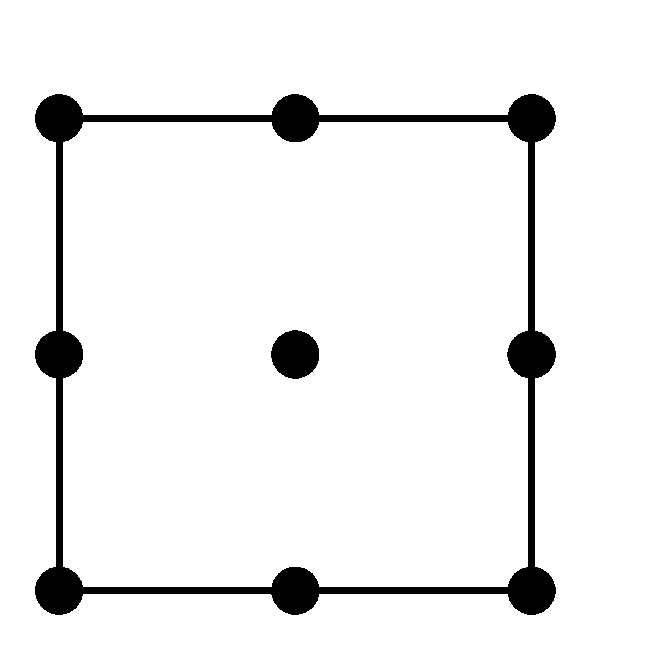
\includegraphics[width=\textwidth]{graph/nodes_q2}
    \end{column}
    \begin{column}{.65\textwidth}
      \begin{itemize}
      \item Tensor product polynomials
        \begin{gather*}
          Q_k = \bigl\{p(x)q(y)\big|
          p,q\in P_2\bigr\}
        \end{gather*}
      \item Quadrature for node functionals
        \begin{itemize}
        \item Others possible, e.g. moments
        \end{itemize}
      \end{itemize}
    \end{column}
  \end{columns}
\end{frame}

\begin{frame}
  \frametitle{Example: $Q_2$ shape functions}
  \begin{center}
    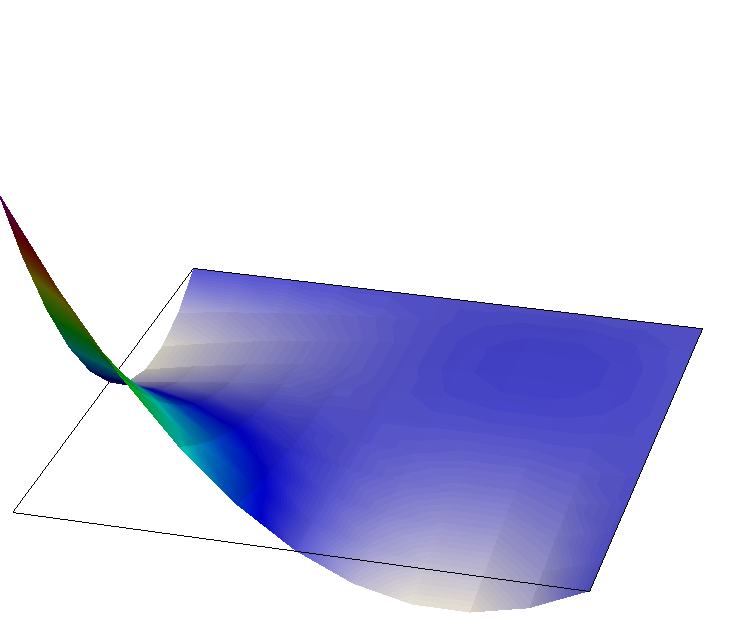
\includegraphics[height=.3\textheight]{graph/shape0}
    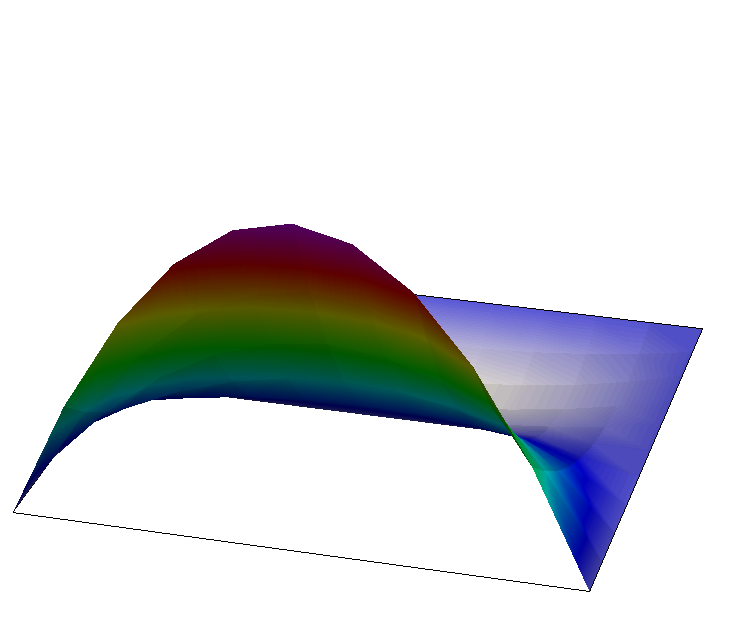
\includegraphics[height=.3\textheight]{graph/shape1}
    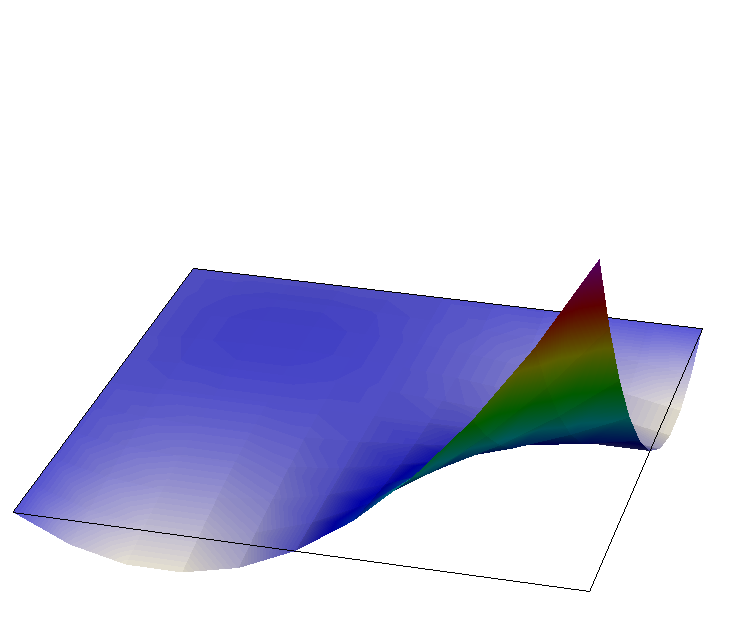
\includegraphics[height=.3\textheight]{graph/shape2}

    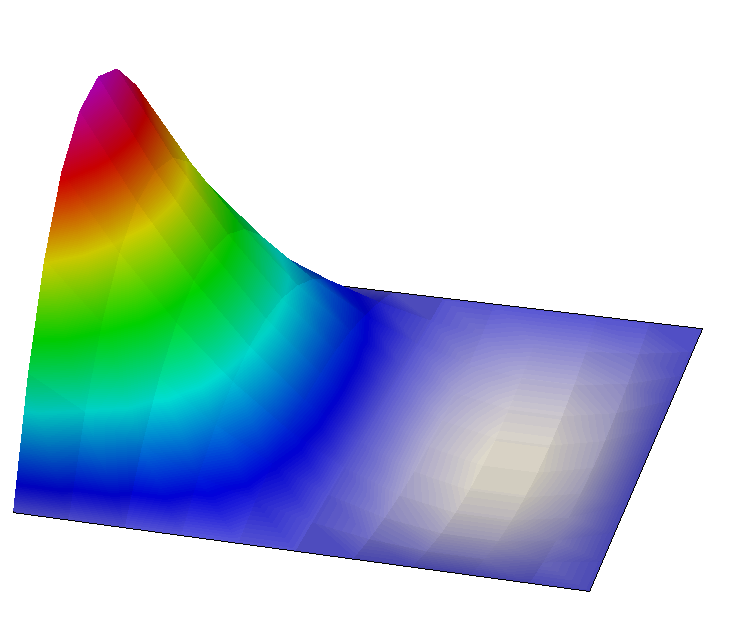
\includegraphics[height=.3\textheight]{graph/shape3}
    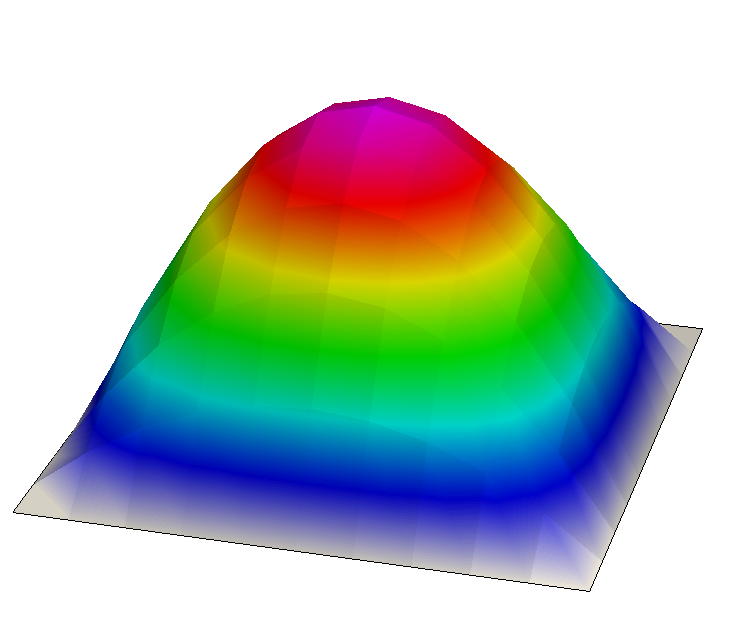
\includegraphics[height=.3\textheight]{graph/shape4}
    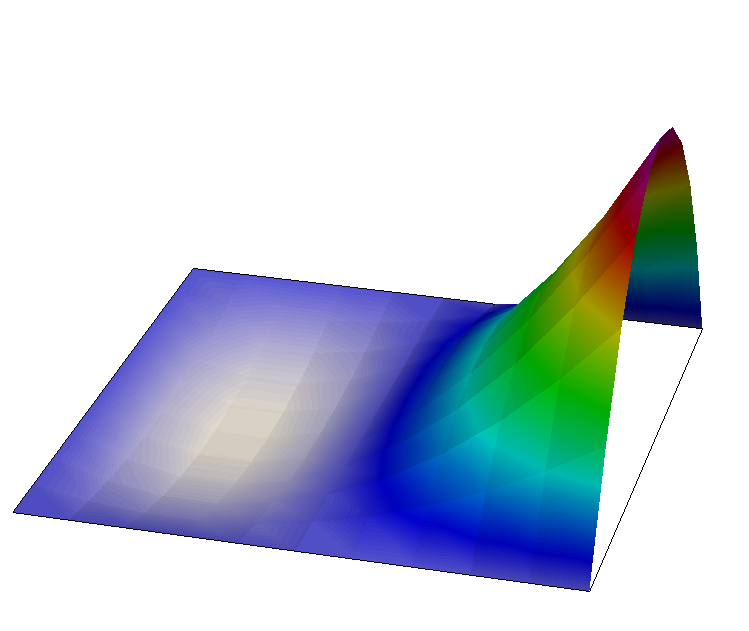
\includegraphics[height=.3\textheight]{graph/shape5}

    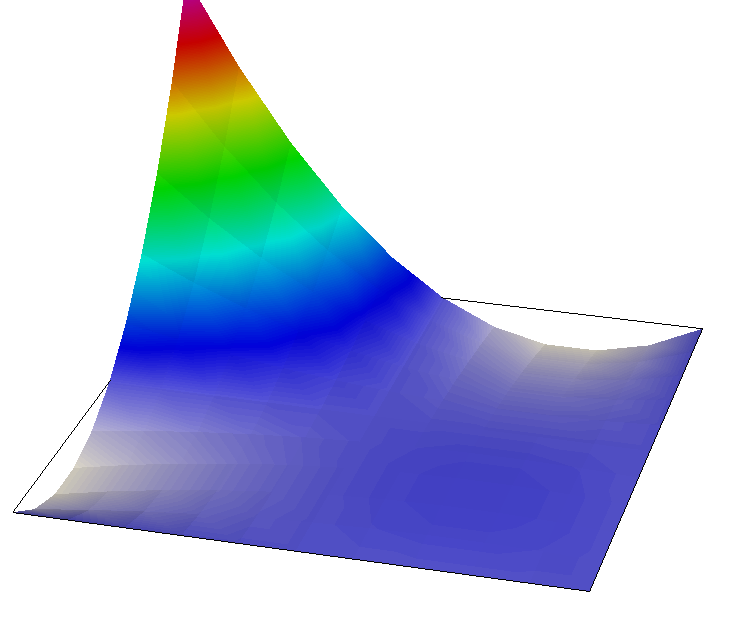
\includegraphics[height=.3\textheight]{graph/shape6}
    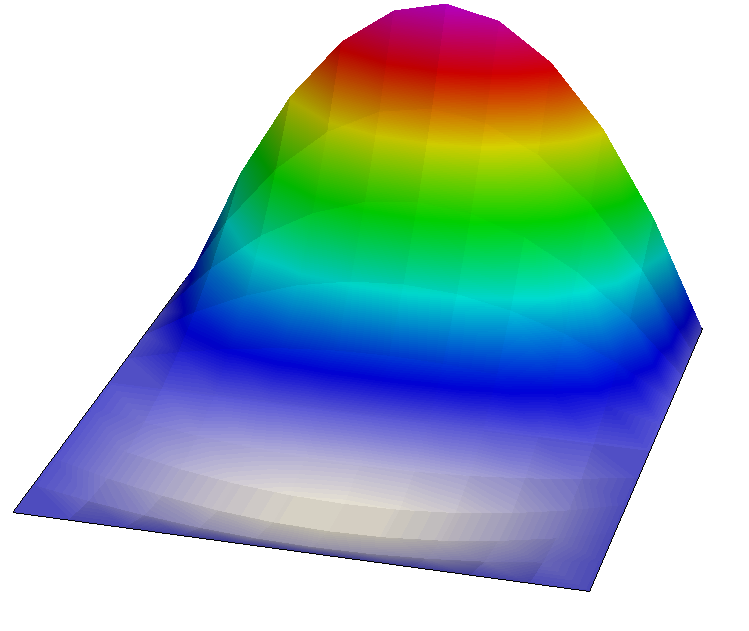
\includegraphics[height=.3\textheight]{graph/shape7}
    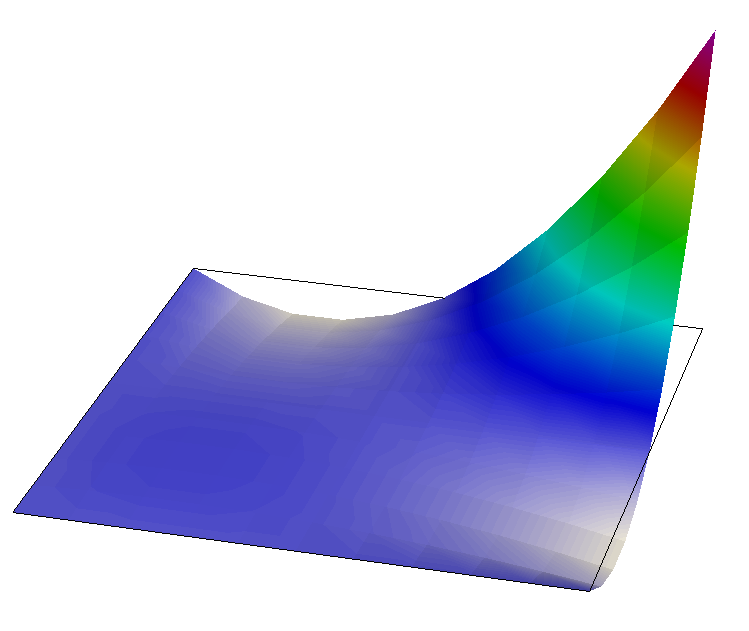
\includegraphics[height=.3\textheight]{graph/shape8}
  \end{center}
\end{frame}

%%%%%%%%%%%%%%%%%%%%%%%%%%%%%%%%%%%%%%%%%%%%%%%%%%%%%%%%%%%%%%%%%%%%%%
\begin{frame}
  \frametitle{Global finite element spaces}
  \begin{itemize}
  \item Throw a mesh over the domain $\Omega$
  \item Concatenate the spaces $P_K$ to obtain discrete space $V_h$
  \item Eliminate identified degrees of freedom and count globally
  \item ``Glued'' shape functions become basis functions $\phi_i$
    \begin{itemize}
    \item $i$ is a ``global'' index unique for the whole mesh
    \end{itemize}
  \end{itemize}
\end{frame}

% TODO: Q2 basis functions

\begin{frame}
  \frametitle{Example: $Q_2$ continuous basis (selection)}
  \begin{center}
    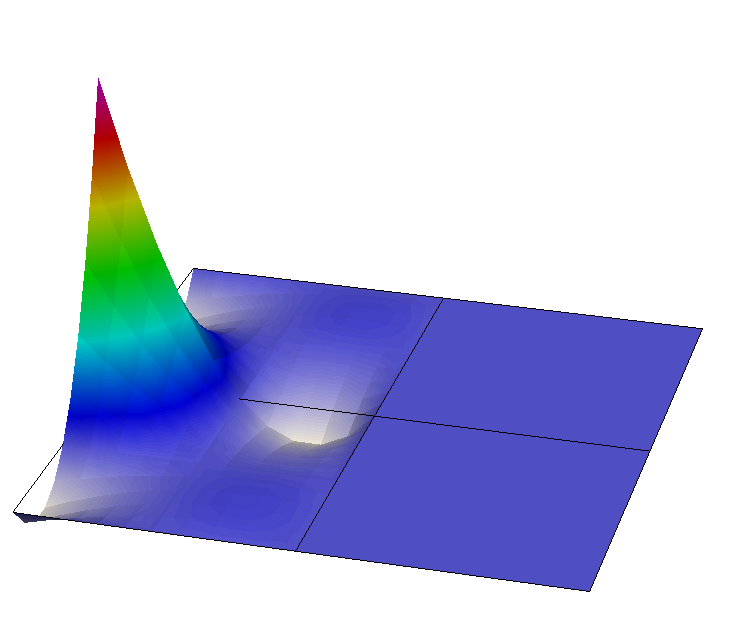
\includegraphics[height=.27\textheight]{graph/cgbasis1-02}
    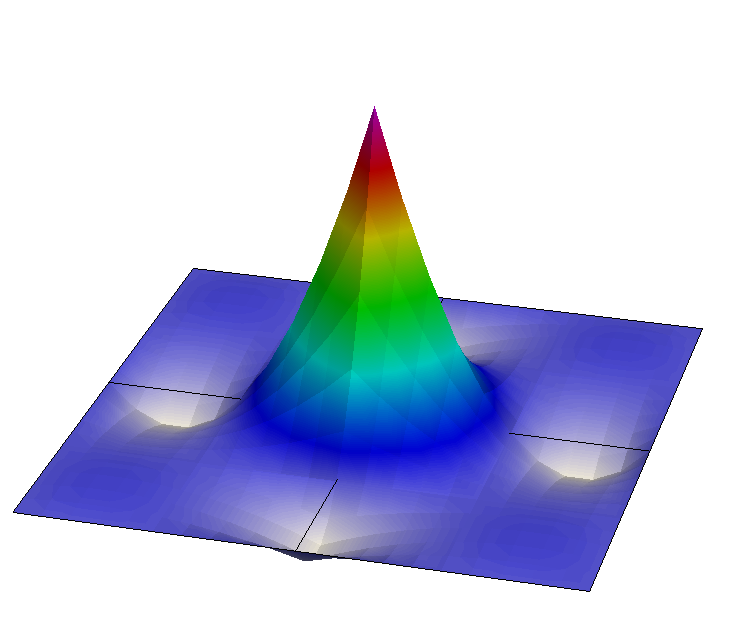
\includegraphics[height=.27\textheight]{graph/cgbasis1-03}
    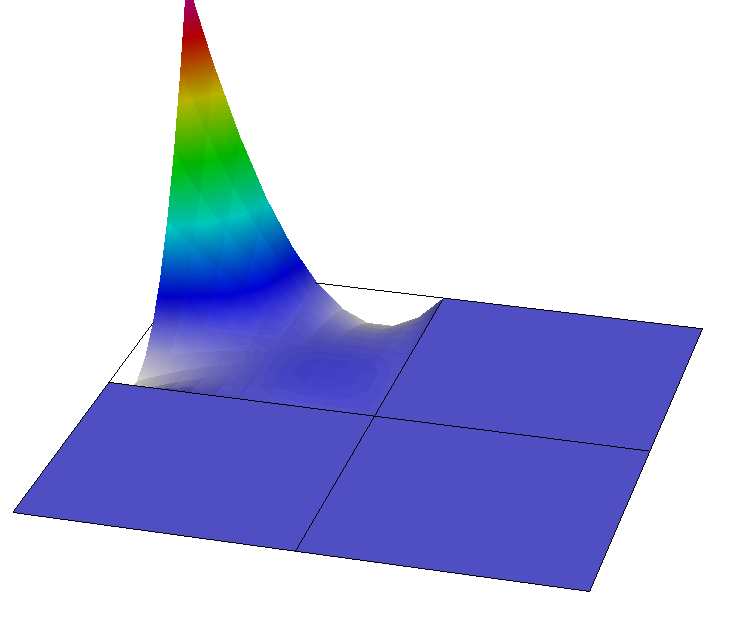
\includegraphics[height=.27\textheight]{graph/cgbasis1-15}
    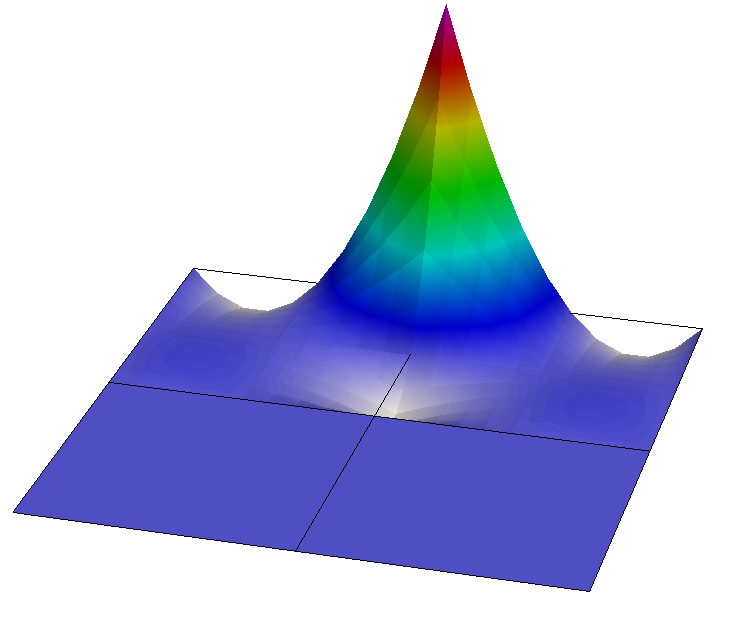
\includegraphics[height=.27\textheight]{graph/cgbasis1-16}

    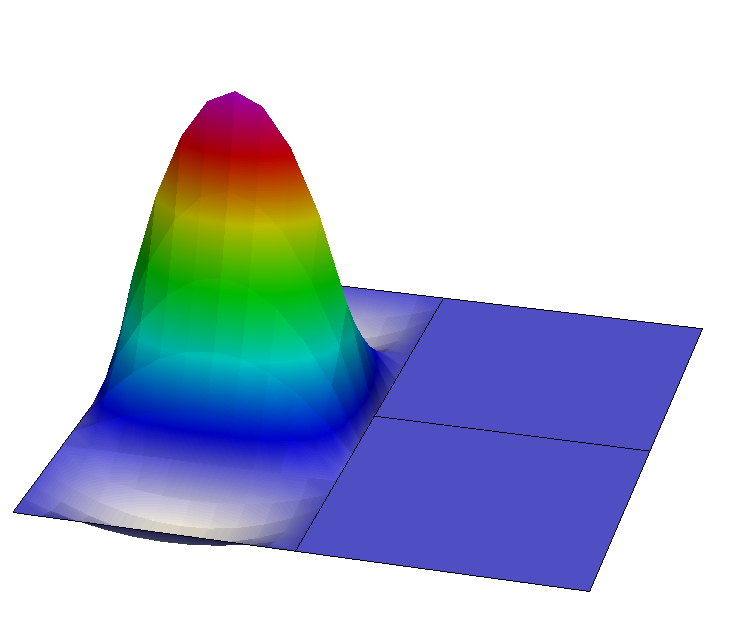
\includegraphics[height=.27\textheight]{graph/cgbasis1-07}
    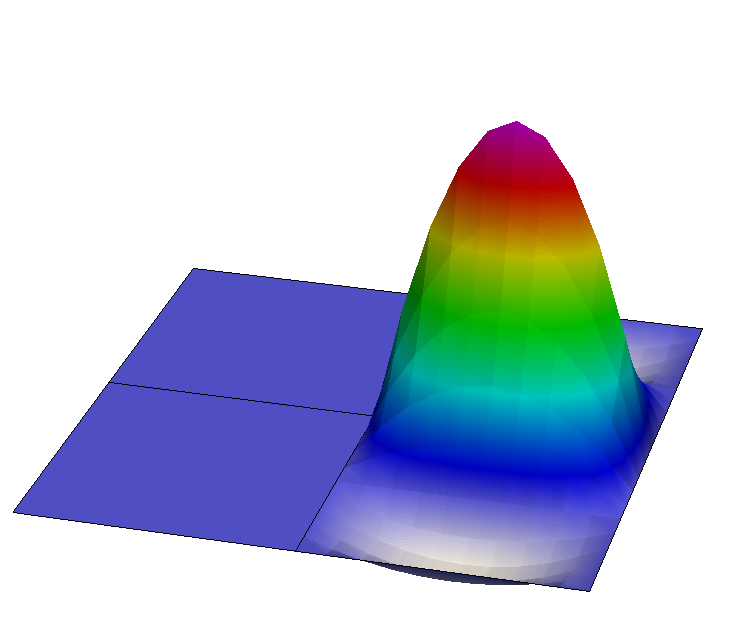
\includegraphics[height=.27\textheight]{graph/cgbasis1-13}
    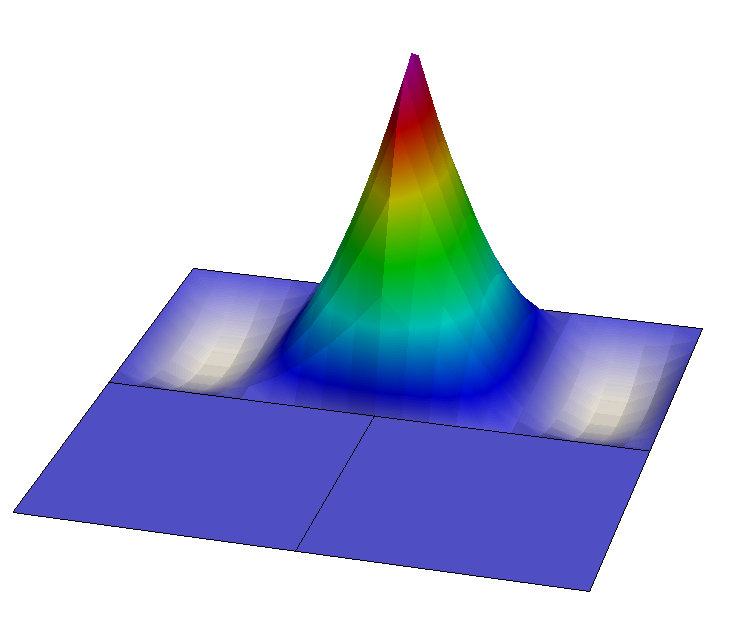
\includegraphics[height=.27\textheight]{graph/cgbasis1-18}
    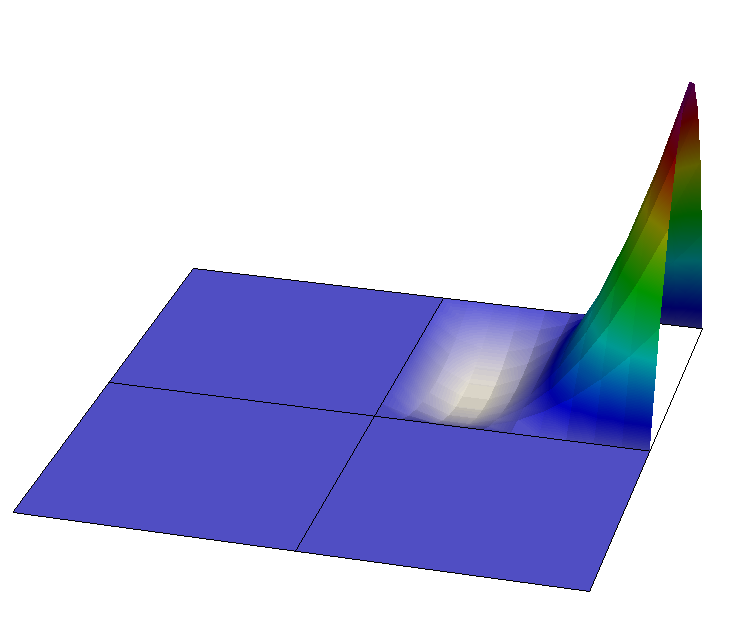
\includegraphics[height=.27\textheight]{graph/cgbasis1-22}

    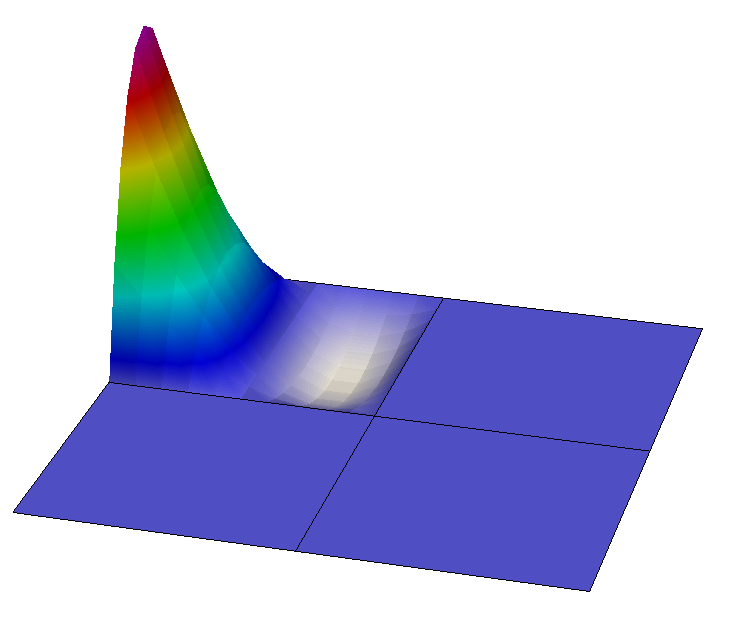
\includegraphics[height=.27\textheight]{graph/cgbasis1-17}
    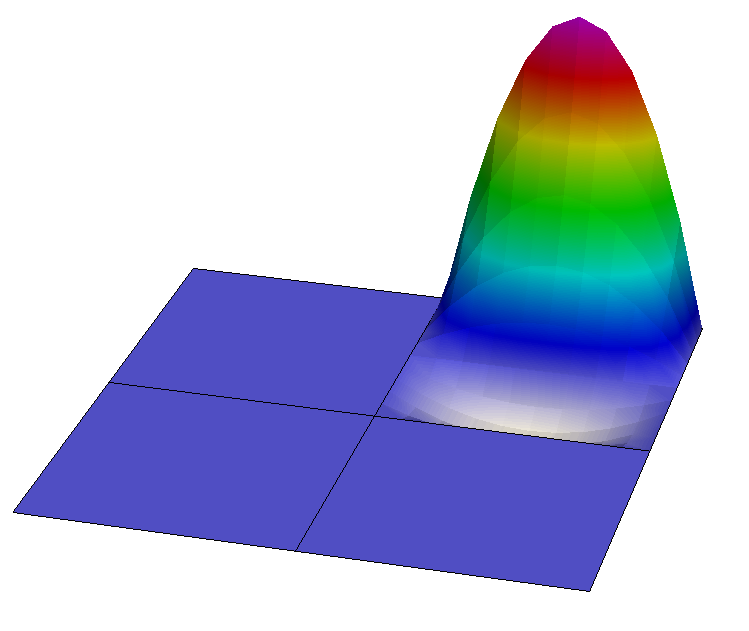
\includegraphics[height=.27\textheight]{graph/cgbasis1-23}
    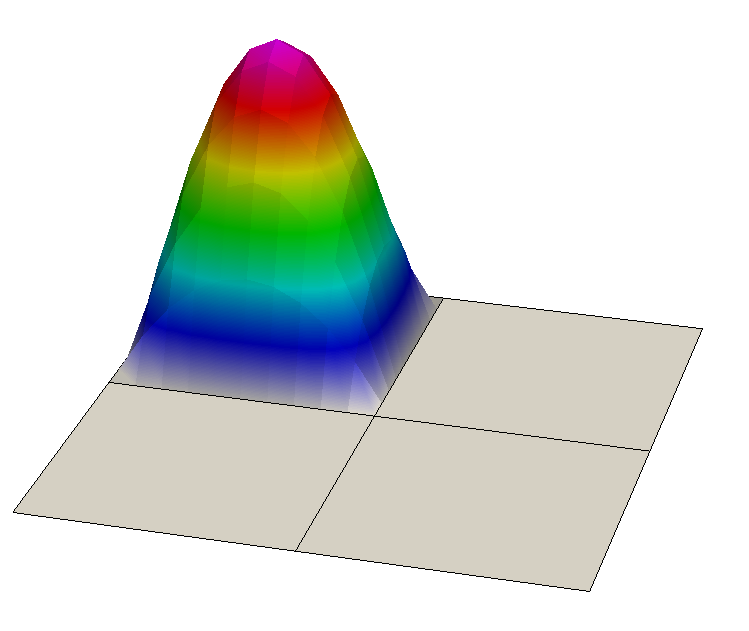
\includegraphics[height=.27\textheight]{graph/cgbasis1-20}
    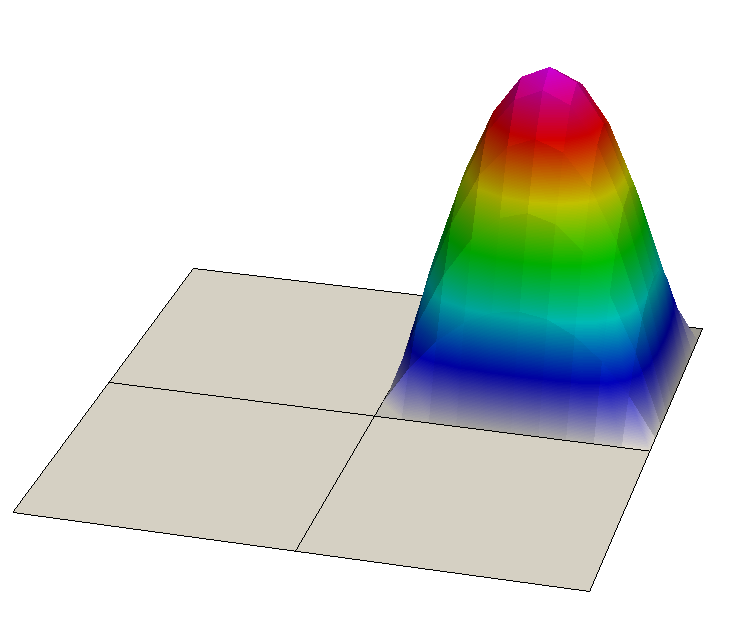
\includegraphics[height=.27\textheight]{graph/cgbasis1-24}
  \end{center}
\end{frame}

\begin{frame}
  \frametitle{Example: $Q_2$ discontinuous basis (selection)}
  \begin{center}
    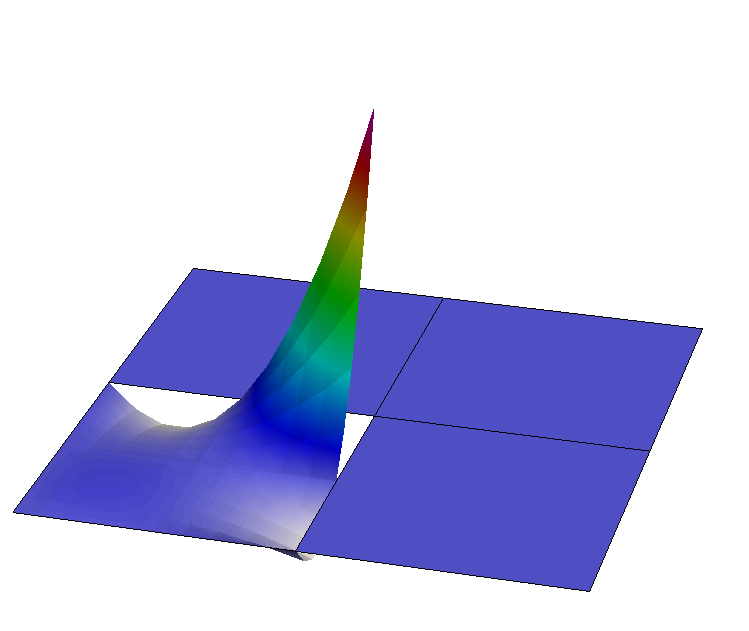
\includegraphics[height=.27\textheight]{graph/dgbasis1-08}
    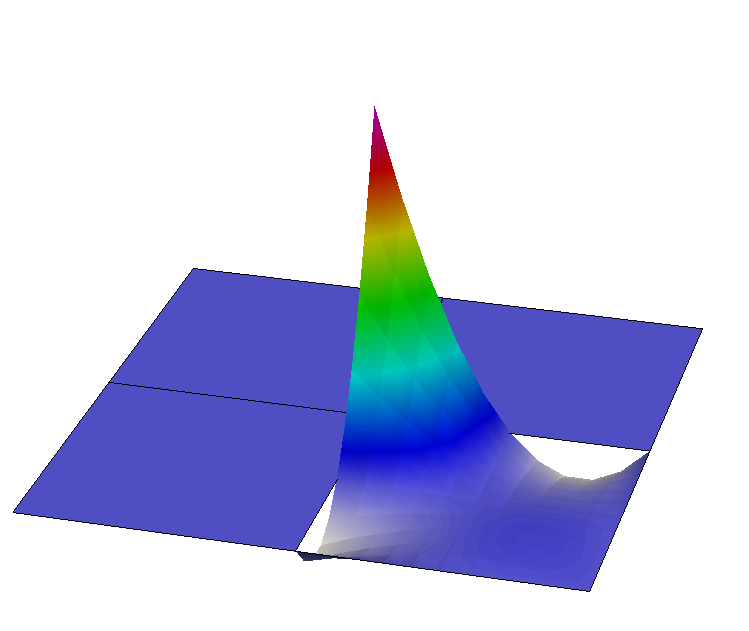
\includegraphics[height=.27\textheight]{graph/dgbasis1-15}
    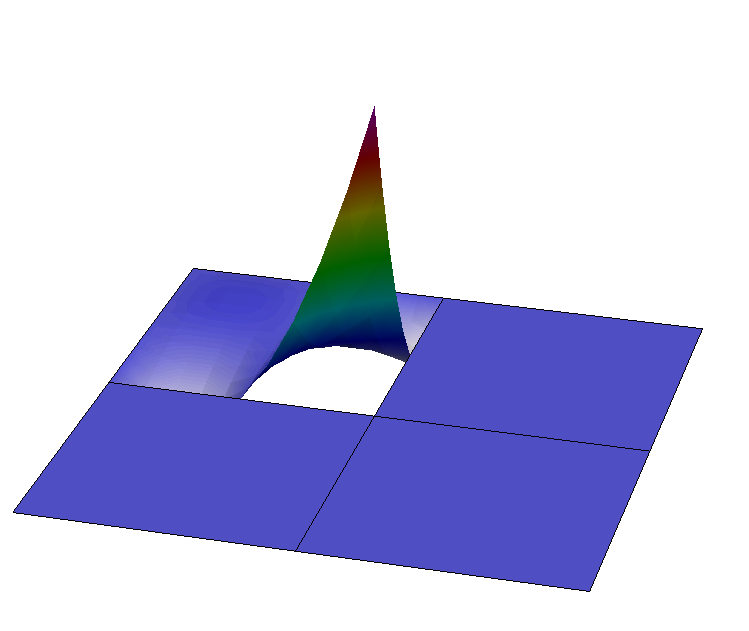
\includegraphics[height=.27\textheight]{graph/dgbasis1-20}
    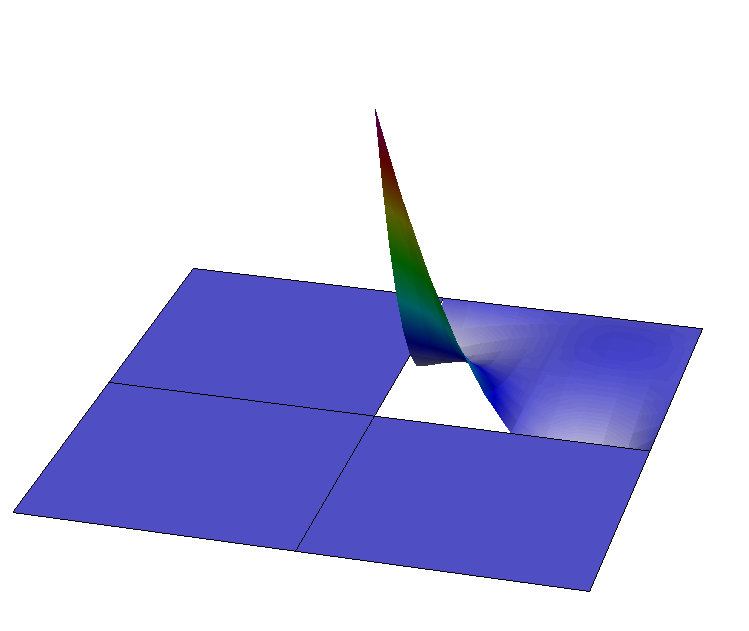
\includegraphics[height=.27\textheight]{graph/dgbasis1-27}

    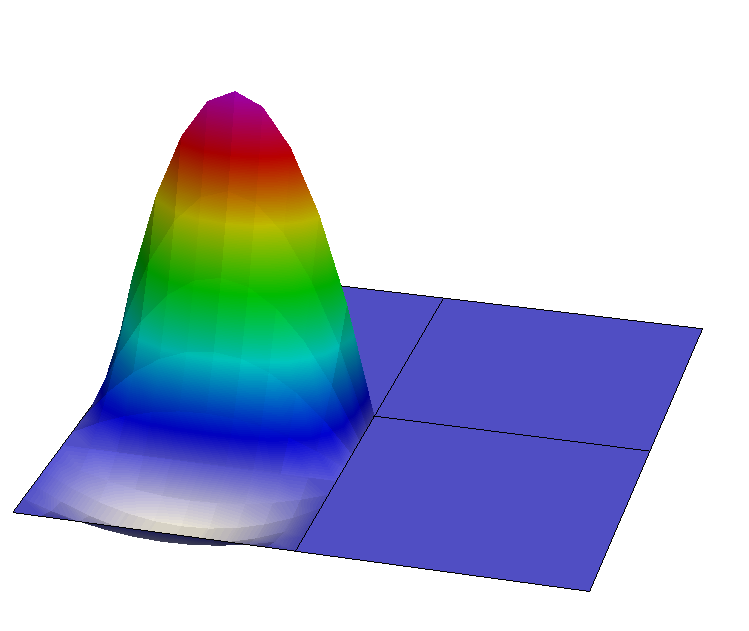
\includegraphics[height=.27\textheight]{graph/dgbasis1-07}
    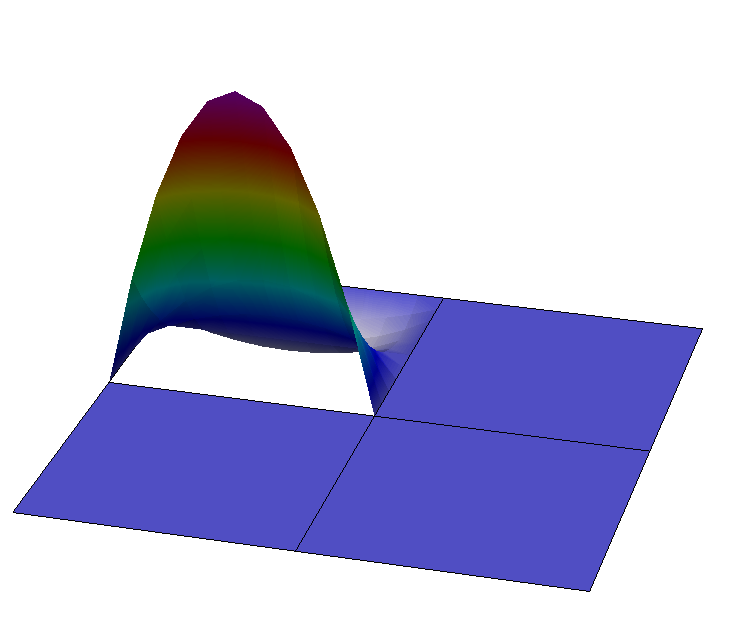
\includegraphics[height=.27\textheight]{graph/dgbasis1-19}
    \includegraphics[height=.27\textheight]{graph/dgbasis1-23}
    \includegraphics[height=.27\textheight]{graph/dgbasis1-30}

    \includegraphics[height=.27\textheight]{graph/dgbasis1-26}
    \includegraphics[height=.27\textheight]{graph/dgbasis1-33}
    \includegraphics[height=.27\textheight]{graph/dgbasis1-24}
    \includegraphics[height=.27\textheight]{graph/dgbasis1-22}
  \end{center}
\end{frame}

%%%%%%%%%%%%%%%%%%%%%%%%%%%%%%%%%%%%%%%%%%%%%%%%%%%%%%%%%%%%%%%%%%%%%% 
\begin{frame}
  \frametitle{Finite Element Spaces in deal.II}
  \begin{itemize}
  \item Meshes are handled by \lstinline!Triangulation<dim,sdim>!
  \item Classes derived from \lstinline!FiniteElement<dim,sdim>!
    define ``shape function space'' and ``node values''
  \item \lstinline!DoFHandler<dim,sdim>! administers the ``global
    finite element space''
  \end{itemize}
  \begin{block}{}
    \lstinputlisting{code/generic_setup.cc}
  \end{block}
\end{frame}

%%%%%%%%%%%%%%%%%%%%%%%%%%%%%%%%%%%%%%%%%%%%%%%%%%%%%%%%%%%%%%%%%%%%%%
%%%%%%%%%%%%%%%%%%%%%%%%%%%%%%%%%%%%%%%%%%%%%%%%%%%%%%%%%%%%%%%%%%%%%%
\subsection{Weak formulation}

%%%%%%%%%%%%%%%%%%%%%%%%%%%%%%%%%%%%%%%%%%%%%%%%%%%%%%%%%%%%%%%%%%%%%%
\begin{frame}
  \frametitle{A model problem}
  \begin{itemize}
  \item Poisson problem with Dirichlet boundary conditions
    \begin{gather*}
      -\Delta u = f \text{ in }\Omega,\qquad u=0 \text{ on }\partial\Omega.
    \end{gather*}
  \item Weak formulation: find $u\in V = H^1_0(\Omega)$ such that
    \begin{gather*}
      \int_\Omega \nabla u\cdot \nabla v \,dx
      =
      \int_\Omega fv\,dx
      \quad\forall v\in V
    \end{gather*}
  \end{itemize}
\end{frame}

%%%%%%%%%%%%%%%%%%%%%%%%%%%%%%%%%%%%%%%%%%%%%%%%%%%%%%%%%%%%%%%%%%%%%%
\begin{frame}
  \frametitle{Weak form for FEM}
  \begin{itemize}
  \item Find $u\in V_h$ such that
    \begin{gather*}
      \int_\Omega \nabla u\cdot \nabla v \,dx
      =
      \int_\Omega fv\,dx
      \quad\forall v\in V_h
    \end{gather*}
  \item The weak formulation
    \begin{gather*}
      a(u,v) = f(v)
    \end{gather*}
  \item The discrete problem (linear algebra)
    \begin{gather*}
      \only<2->{v^T} Au =  \only<2->{v^T}f
    \end{gather*}
  \end{itemize}
  \pause
  \begin{block}{Warning!!!}
    The order of trial and test space is reverted!
    \begin{gather*}
      a_{\red ij} = %\sum_{K \in \mathbb T_h}
      a(\phi_j, \phi_i)
    \end{gather*}
  \end{block}
\end{frame}

\begin{frame}
  \frametitle{Implementation of the integrals}
  \begin{itemize}
  \item Split the integrals
    \begin{gather*}
      \int_\Omega \bullet \, dx = \sum_{K \in \T_h}\int_K \bullet \; dx
    \end{gather*}
  \item Only small number of shape functions get integrated
    \begin{itemize}
    \item Complexity linear in number of cells!
    \end{itemize}
  \item Local integrals are simple and computed by quadrature
    \begin{gather*}
      a_{ij}^K = \int_K \nabla \psi_j \cdot \nabla \psi_i\,d x
    \end{gather*}
  \item Mapping from local to global indices to add cell matrices $A_K$
  \end{itemize}
\end{frame}

%%%%%%%%%%%%%%%%%%%%%%%%%%%%%%%%%%%%%%%%%%%%%%%%%%%%%%%%%%%%%%%%%%%%%%
%%%%%%%%%%%%%%%%%%%%%%%%%%%%%%%%%%%%%%%%%%%%%%%%%%%%%%%%%%%%%%%%%%%%%%
\subsection{Solving the discrete problems}

%%%%%%%%%%%%%%%%%%%%%%%%%%%%%%%%%%%%%%%%%%%%%%%%%%%%%%%%%%%%%%%%%%%%%%
\begin{frame}
  \frametitle{Sparse matrices}
  \begin{itemize}
  \item Matrices from finite element discretizations tend to be large
    \begin{itemize}
    \item $10^6$ to $10^9$ rows are common nowadays
    \item Example: $Q_1$ on a $100^3$ grid in 3D
    \end{itemize}
  \item Only basis functions with common support generate entries
    \begin{itemize}
    \item Only functions on a cell
    \item Very few entries per line
    \item Entries are scattered according to the mesh and numbering
    \end{itemize}
  \end{itemize}
\end{frame}

%%%%%%%%%%%%%%%%%%%%%%%%%%%%%%%%%%%%%%%%%%%%%%%%%%%%%%%%%%%%%%%%%%%%%%
\begin{frame}
  \frametitle{Effort for linear solvers}
  Example: uniform mesh of $100^3$ cells, $10^9$ flops/sec
  \begin{itemize}
  \item<+-> Gauß elimination, $LU$ decomposition
    \only<2->{: 10 years}
    \only<1>{\begin{itemize}
    \item Effort: $n^3/3 + \mathcal O(n^2)$ flops
    \item Example: $100^9/3 = 10^{18}/3 \text{flops} \approx 10^9/3 \text{sec}
      \approx 10^4/3 \text{days} \approx 10  \text{years}$
    \end{itemize}}
  \item<+-> Banded version, skyline solver
    \only<3->{: 8 hours}
    \only<2>{\begin{itemize}
    \item Effort: $n/3 (n^{2/3})^2 + \mathcal O(n^2)
      \approx n^{7/3}$ flops
    \item Example: $100^7/3 = 10^{14}/3 \text{flops}
      \approx 10^5/3 \text{sec}
      \approx 8 \text{hours}$
    \end{itemize}}
  \item<+-> Cramer's rule, Laplace expansion
    \only<4->{: $\infty$}
    \only<3>{\begin{itemize}
    \item Effort: $n!$
    \item Example: $100! \approx 10^{55,000} \text{years}$
    \end{itemize}}
  \item<+-> Iterative methods: matrix vector multiplication and
    preconditioning
    \begin{itemize}
    \item Effort: number of nonzero entries plus preconditioning
      in each step
    \item Example: $7\cdot 10^6\text{flops} \approx 0.1
      \text{sec}$ per step
    \item Mulitgrid: times 10?
    \end{itemize}
  \end{itemize}
\end{frame}

%%%%%%%%%%%%%%%%%%%%%%%%%%%%%%%%%%%%%%%%%%%%%%%%%%%%%%%%%%%%%%%%%%%%%%
\begin{frame}
  \frametitle{Sparsity pattern}
  \begin{itemize}
  \item Enumerate the positions in a line where nonzero entries of the matrix may be
  \end{itemize}
  \begin{center}
    \includegraphics[width=.4\textwidth]{graph/step-2-sparsity-1}
    \includegraphics[width=.4\textwidth]{graph/step-2-sparsity-2}
  \end{center}
  \begin{itemize}
  \item All matrices for the same finite element space have the same sparsity pattern
  \end{itemize}
\end{frame}

\subsection{Problems}
\begin{frame}
  \frametitle{Exercises: finite element spaces and sparsity}
  {\footnotesize{\url{http://www.dealii.org/\dealrelease/doxygen/deal.II/step_2.html}}}
  \begin{itemize}
  \item Additional information:
    \begin{itemize}
    \item \texttt{SparsityPattern::bandwidth()}
    \item \texttt{SparsityPattern::n\_nonzero\_elements()}
    \end{itemize}
  \item Problems: study how these numbers depend on
    \begin{itemize}
    \item finite element degree
    \item mesh refinement
    \item space dimension
    \item Choice of
      \begin{itemize}
      \item \lstinline!FE_Q(k) ! $k=1,2,3$
      \item \lstinline!FE_DGQ(k) ! $k=0,1,2,3$
      \item \lstinline!FE_DGP(k) ! $k=0,1,2,3$
      \item \lstinline!FE_Nedelec(k) ! $k=1,2$
      \end{itemize}
    \end{itemize}
  \end{itemize}
\end{frame}


%%% Local Variables: 
%%% mode: latex
%%% TeX-master: "slides"
%%% End: 


\begin{frame}
  \begin{center}
      End of part 1
  \end{center}
\end{frame}

%%%%%%%%%%%%%%%%%%%%%%%%%%%%%%%%%%%%%%%%%%%%%%%%%%%%%%%%%%%%%%%%%%%%%% 
%%%%%%%%%%%%%%%%%%%%%%%%%%%%%%%%%%%%%%%%%%%%%%%%%%%%%%%%%%%%%%%%%%%%%% 
%\section{Main features}
%\frame{\tableofcontents[currentsection,hideothersubsections]}
%% $Id: features.tex 3667 2013-01-12 21:41:48Z kanschat $

%%%%%%%%%%%%%%%%%%%%%%%%%%%%%%%%%%%%%%%%%%%%%%%%%%%%%%%%%%%%%%%%%%%%%% 
\subsection{Mesh handling}
\begin{frame}
  \frametitle{Mesh handling}
  \begin{itemize}
  \item deal.II uses meshes with ``tensor product cells''
    \begin{itemize}
    \item quadrilaterals in 2D
    \item mapped hexahedra in 3D
    \end{itemize}
  \item Mappings of arbitrary order
  \item support for dimension independent programming
  \item local refinement with ``hanging nodes''
    \begin{center}
      \includegraphics[height=.25\textheight]{graph/hanging}
    \end{center}
  \item storage of mesh hierarchy for multigrid
  \end{itemize}
\end{frame}

%%%%%%%%%%%%%%%%%%%%%%%%%%%%%%%%%%%%%%%%%%%%%%%%%%%%%%%%%%%%%%%%%%%%%% 
\subsection{Shape functions}
\begin{frame}
  \frametitle{Shape functions}
  \begin{itemize}
  \item $H^1$-conforming $Q_k$
  \item $H^{\text{div}}$-conforming RT$_k$, BDM$_k$
  \item $H^{\text{curl}}$-conforming Nedelec$_k$ (first family)
  \item discontinuous $Q_k$, $P_k$, vector elements
  \item support for implementation of further elements
  \end{itemize}
\end{frame}

%%%%%%%%%%%%%%%%%%%%%%%%%%%%%%%%%%%%%%%%%%%%%%%%%%%%%%%%%%%%%%%%%%%%%% 
\subsection{Degrees of freedom}
\begin{frame}
  \frametitle{Degrees of freedom}
  \begin{itemize}
  \item Element ``topology'' gets converted to ``global degrees
    of freedom''
  \item Generalized $hp$-methods
  \item Constraint operators for hanging nodes
  \item Level hierarchies of arbitrary elements
  \item Generic iterators to build matrices on cells and faces
  \end{itemize}
\end{frame}

%%%%%%%%%%%%%%%%%%%%%%%%%%%%%%%%%%%%%%%%%%%%%%%%%%%%%%%%%%%%%%%%%%%%%% 
\subsection{Systems of PDE}
\begin{frame}
  \frametitle{Systems of PDE}
  \begin{itemize}
  \item ``System elements'' simplify the implementation of systems of
    PDE
    \begin{itemize}
    \item Most data handling like for single equations
    \item Only local integrators have to change
    \end{itemize}
  \item Block vectors allow separation of equations
    \begin{itemize}
    \item Block preconditioners
    \item Projection schemes
    \end{itemize}
  \end{itemize}
\end{frame}

%%%%%%%%%%%%%%%%%%%%%%%%%%%%%%%%%%%%%%%%%%%%%%%%%%%%%%%%%%%%%%%%%%%%%% 
\subsection{Linear algebra}
\begin{frame}
  \frametitle{Linear algebra}
  \begin{itemize}
  \item Vectors and sparse matrices
  \item Elimination of hanging nodes
  \item Krylov space solvers: cg, GMRES, MinRes, Bicgstab, TFQMR
  \item Point and block relaxation
    \pause
  \item Multilevel support
  \item Block systems and Schur complements
    \pause
  \item Umfpack
  \item Interfaces to Trilinos, Lapack, Petsc, Slepc
    \pause
  \item Support for matrix free linear algebra work in progress
  \end{itemize}
\end{frame}

%%%%%%%%%%%%%%%%%%%%%%%%%%%%%%%%%%%%%%%%%%%%%%%%%%%%%%%%%%%%%%%%%%%%%% 
\subsection{Pre- and postprocessing}
\begin{frame}
  \frametitle{Pre- and postprocessing}
  \begin{itemize}
  \item<+-> Input drivers for several grid generators
    \begin{itemize}
    \item BAMG, MGF, GMSH, Salome, Cubit
    \item Graphic formats: UCD, Tecplot
    \end{itemize}
  \item<+-> Graphical output split into cell patches
    \begin{itemize}
    \item Drivers for VTK, UCD, OpenDX, gnuplot, Postscript, Tecplot, SVG
    \item Output for higher order elements
    \item New backends easily implemented
    \end{itemize}
  \end{itemize}
\end{frame}

%%%%%%%%%%%%%%%%%%%%%%%%%%%%%%%%%%%%%%%%%%%%%%%%%%%%%%%%%%%%%%%%%%%%%%
\begin{frame}
  \frametitle{The main classes}
  \centering
  \includegraphics[height=.99\textheight]{graph/structure}
\end{frame}

%%%%%%%%%%%%%%%%%%%%%%%%%%%%%%%%%%%%%%%%%%%%%%%%%%%%%%%%%%%%%%%%%%%%%%
\begin{frame}
  \frametitle{The tutorial structure}

  \centering
  \includegraphics[height=.99\textheight]{graph/tutorial}

\end{frame}


%%% Local Variables: 
%%% mode: latex
%%% TeX-master: "slides"
%%% End: 


%%% Local Variables: 
%%% mode: latex
%%% TeX-master: "slides"
%%% End: 

%%%%%%%%%%%%%%%%%%%%%%%%%%%%%%%%%%%%%%%%%%%%%%%%%%%%%%%%%%%%%%%%%%%%%%
%%%%%%%%%%%%%%%%%%%%%%%%%%%%%%%%%%%%%%%%%%%%%%%%%%%%%%%%%%%%%%%%%%%%%%
%%%%%%%%%%%%%%%%%%%%%%%%%%%%%%%%%%%%%%%%%%%%%%%%%%%%%%%%%%%%%%%%%%%%%%
%%%%%%%%%%%%%%%%%%%%%%%%%%%%%%%%%%%%%%%%%%%%%%%%%%%%%%%%%%%%%%%%%%%%%%
\part{Guided tour through selected tutorials}

\section*{Part 2}
\begin{frame}
  \frametitle{Guided tour through selected tutorials}
  \tableofcontents[hideallsubsections]
\end{frame}

%%%%%%%%%%%%%%%%%%%%%%%%%%%%%%%%%%%%%%%%%%%%%%%%%%%%%%%%%%%%%%%%%%%%%%
%%%%%%%%%%%%%%%%%%%%%%%%%%%%%%%%%%%%%%%%%%%%%%%%%%%%%%%%%%%%%%%%%%%%%%
%\section[Example]{An example program}
%% $Id: example.tex 2782 2011-07-25 16:39:35Z kanschat $

\lstset{language=C++,
  basicstyle=\scriptsize,%\ttfamily,
  keywordstyle=\bfseries,
  showtabs=false,
  showspaces=false,
  tabsize=2}

\subsection{Tutorial Step 16}
\begin{frame}
  \frametitle{Example: tutorial step 16}
  \begin{itemize}
  \item Solve a Poisson problem
  \item Error estimation and local refinement
  \item Continuous elements with hanging nodes
  \item Multigrid solver
  \end{itemize}
\end{frame}

%%%%%%%%%%%%%%%%%%%%%%%%%%%%%%%%%%%%%%%%%%%%%%%%%%%%%%%%%%%%%%%%%%%%%%
\begin{frame}
  \frametitle{The main class (functions)}
  \lstinputlisting{code/class1.cc}
\end{frame}

%%%%%%%%%%%%%%%%%%%%%%%%%%%%%%%%%%%%%%%%%%%%%%%%%%%%%%%%%%%%%%%%%%%%%%
\begin{frame}
  \frametitle{The main class (data)}
  \lstinputlisting{code/class2.cc}
\end{frame}

%%%%%%%%%%%%%%%%%%%%%%%%%%%%%%%%%%%%%%%%%%%%%%%%%%%%%%%%%%%%%%%%%%%%%%
\begin{frame}
  \frametitle{The main class (multigrid)}
  \lstinputlisting{code/class3.cc}
\end{frame}

%%%%%%%%%%%%%%%%%%%%%%%%%%%%%%%%%%%%%%%%%%%%%%%%%%%%%%%%%%%%%%%%%%%%%%
\begin{frame}
  \frametitle{The main class (declaration)}
  \lstinputlisting[basicstyle=\tiny,numberstyle=\tiny,numbers=left,numbersep=0pt,stepnumber=1]{code/class.cc}
\end{frame}

%%%%%%%%%%%%%%%%%%%%%%%%%%%%%%%%%%%%%%%%%%%%%%%%%%%%%%%%%%%%%%%%%%%%%%
\begin{frame}
  \frametitle{The constructor}
  \lstinputlisting{code/constructor.cc}
\end{frame}

%%%%%%%%%%%%%%%%%%%%%%%%%%%%%%%%%%%%%%%%%%%%%%%%%%%%%%%%%%%%%%%%%%%%%%
\begin{frame}
  \frametitle{Setting up the system}
  \lstinputlisting{code/setup.cc}
\end{frame}

%%%%%%%%%%%%%%%%%%%%%%%%%%%%%%%%%%%%%%%%%%%%%%%%%%%%%%%%%%%%%%%%%%%%%%
\begin{frame}
  \frametitle{Boundary and hanging node constraints}
  \lstinputlisting{code/constraints.cc}
\end{frame}

%%%%%%%%%%%%%%%%%%%%%%%%%%%%%%%%%%%%%%%%%%%%%%%%%%%%%%%%%%%%%%%%%%%%%%
\begin{frame}[t]
  \frametitle{Assembling the matrix}
  \lstinputlisting{code/matrix.cc}
\end{frame}

%%%%%%%%%%%%%%%%%%%%%%%%%%%%%%%%%%%%%%%%%%%%%%%%%%%%%%%%%%%%%%%%%%%%%%
\begin{frame}[t]
  \frametitle{Assembling the multilevel matrices}
  \lstinputlisting{code/mgmatrix.cc}
\end{frame}

%%%%%%%%%%%%%%%%%%%%%%%%%%%%%%%%%%%%%%%%%%%%%%%%%%%%%%%%%%%%%%%%%%%%%%
\begin{frame}[t]
  \frametitle{Assembling the right hand side}
  \lstinputlisting{code/rhs.cc}
\end{frame}

%%%%%%%%%%%%%%%%%%%%%%%%%%%%%%%%%%%%%%%%%%%%%%%%%%%%%%%%%%%%%%%%%%%%%%
\begin{frame}[t]
  \frametitle{Solving the linear system}
  \lstinputlisting{code/solve2.cc}
\end{frame}

%%%%%%%%%%%%%%%%%%%%%%%%%%%%%%%%%%%%%%%%%%%%%%%%%%%%%%%%%%%%%%%%%%%%%%
\begin{frame}[t]
  \frametitle{Setting up the preconditioner}
  \lstinputlisting[basicstyle=\tiny]{code/solve1.cc}
\end{frame}

%%%%%%%%%%%%%%%%%%%%%%%%%%%%%%%%%%%%%%%%%%%%%%%%%%%%%%%%%%%%%%%%%%%%%%
\begin{frame}[t]
  \frametitle{Output}
  \lstinputlisting{code/output.cc}
\end{frame}

%%%%%%%%%%%%%%%%%%%%%%%%%%%%%%%%%%%%%%%%%%%%%%%%%%%%%%%%%%%%%%%%%%%%%%
\begin{frame}[t]
  \frametitle{The outer loop}
  \lstinputlisting{code/run.cc}
\end{frame}

%%%%%%%%%%%%%%%%%%%%%%%%%%%%%%%%%%%%%%%%%%%%%%%%%%%%%%%%%%%%%%%%%%%%%%
\begin{frame}[t]
  \frametitle{The function ``main''}
  \lstinputlisting{code/main.cc}
\end{frame}

%%%%%%%%%%%%%%%%%%%%%%%%%%%%%%%%%%%%%%%%%%%%%%%%%%%%%%%%%%%%%%%%%%%%%%
\begin{frame}[t]
  \frametitle{The cell matrix}
  \lstinputlisting{code/cell_matrix.cc}
\end{frame}

%%%%%%%%%%%%%%%%%%%%%%%%%%%%%%%%%%%%%%%%%%%%%%%%%%%%%%%%%%%%%%%%%%%%%%
\begin{frame}[t]
  \frametitle{The cell matrix}
  \lstinputlisting{code/cell_matrix2.cc}
\end{frame}

%%% Local Variables: 
%%% mode: latex
%%% TeX-master: "slides"
%%% End: 


%\begin{frame}
  \frametitle{Step 1 Problems: meshes}
  \begin{enumerate}
    \item Locally refined square mesh
    \begin{enumerate}
    \item Create a mesh for the square $[-1,1]^2$ and refine once globally.
    \item On a given mesh refine all cells with at least one vertex in
      the cicle of radius $1/8$ around the origin. Repeat 6 times to
      resolve the circle.
    \item Visualize the result (gnuplot, SVG, or VTK). Use the online
      documentation to find options. Play!
    \end{enumerate}
  \item Generate a half open shell. How do inner and outer radius
    affect the shape of cells? Visualize!
  \end{enumerate}
\end{frame}

\begin{frame}
  \frametitle{Step 3 Problems: Poisson equation}
  \begin{enumerate}
  \item Solve Helmholtz equation
    \begin{gather*}
      \int \nabla u\cdot\nabla v\,dx - \kappa^2 \int uv\,dx= \int 1v\,dx
    \end{gather*}
    with $\kappa = 1, 4, 10$.
  \item Change the linear solver if necessary
  \item What happens if you refine more?
  \item Change the boundary condition to the natural boundary condition
    \begin{gather*}
      \partial_n u = 0
    \end{gather*}
    on part of the boundary.
  \end{enumerate}
\end{frame}

\begin{frame}
  \frametitle{Problem: Poisson equation, local refinement II}
  \begin{enumerate}
  \item Add a \lstinline!ConstraintMatrix! to your main class and fill it, using
    \begin{itemize}
    \item \lstinline!DoFTools::make_zero_boundary_constraints()!
    \item \lstinline!DoFTools::make_hanging_node_constraints()!
    \end{itemize}
  \item Integrate the bilinear form into a \lstinline!FullMatrix! on
    each cell.
  \item Distribute the cell matrix and cell vector using the
    \lstinline!ConstraintMatrix!
  \item After solving, use \lstinline!ConstraintMatrix::distribute()!
    to get the vector into a format that can be displayed
  \item Use \lstinline!KellyErrorEstimator! on an L-shaped domain for
    adaptive refinement
  \end{enumerate}
Hint: if you get stuck, read the documentation or step 6.
\end{frame}

\begin{frame}
  \frametitle{Problem: Poisson equation, local refinement}
  \begin{enumerate}
  \item Use one of the locally refined meshes from the first set of
    exercises and verify that the solution becomes bad
  \item Add a \lstinline!ConstraintMatrix! to your main class and fill it, using
    \begin{itemize}
    \item \lstinline!DoFTools::make_zero_boundary_constraints()!
    \item \lstinline!DoFTools::make_hanging_node_constraints()!
    \end{itemize}
  \item Integrate the bilinear form into a \lstinline!FullMatrix! on
    each cell.
  \item Distribute the cell matrix and cell vector using the
    \lstinline!ConstraintMatrix!
  \item After solving, use \lstinline!ConstraintMatrix::distribute()!
    to get the vector into a format that can be displayed
  \item Use \lstinline!KellyErrorEstimator! on an L-shaped domain for
    adaptive refinement
  \end{enumerate}
Hint: if you get stuck, read the documentation or step 6.
\end{frame}

\begin{frame}
  \frametitle{Problems}
  \begin{enumerate}
  \item Compare the results with different cycles
    \begin{itemize}
    \item V-cycle
    \item variable V-cycle
    \item W-cycle
    \item F-cycle
    \end{itemize}
  \item Change the number of smoothing steps
  \item Solve Helmholtz equation instead of Poisson
  \item Add advection in $x$-direction
    \begin{itemize}
    \item Beware of a trick that is used for the interface matrices!
    \end{itemize}
  \end{enumerate}
\end{frame}

%%%%%%%%%%%%%%%%%%%%%%%%%%%%%%%%%%%%%%%%%%%%%%%%%%%%%%%%%%%%%%%%%%%%%% 
%%%%%%%%%%%%%%%%%%%%%%%%%%%%%%%%%%%%%%%%%%%%%%%%%%%%%%%%%%%%%%%%%%%%%% 
\section[DG]{Discontinuous Galerkin methods}
\frame{\tableofcontents[currentsection,hideothersubsections]}

%%%%%%%%%%%%%%%%%%%%%%%%%%%%%%%%%%%%%%%%%%%%%%%%%%%%%%%%%%%%%%%%%%%%%%
\subsection{Discontinuous Galerkin methods}

\begin{frame}
  \frametitle{Origin of DG methods}
  \begin{itemize}
  \item Discontinuous Galerkin methods were developed for hyperbolic PDE
    \begin{itemize}
    \item Linear transport: Reed/Hill, LeSaint/Raviart
    \item Nonlinear conservation laws: Cockburn/Shu
    \end{itemize}
  \item They feature basis functions with no continuity across cell boundaries
  \item Soon, an extension to singularly perturbed problems became
    necessary
    \begin{gather*}
      -\varepsilon\Delta u + (w\!\cdot\!\nabla) u = f
    \end{gather*}
  \end{itemize}
\end{frame}

%%%%%%%%%%%%%%%%%%%%%%%%%%%%%%%%%%%%%%%%%%%%%%%%%%%%%%%%%%%%%%%%%%%%%%
\begin{frame}
  \frametitle{DG Methods for elliptic problems}
  \begin{itemize}
  \item Continuity is necessary for $H^1$-conformity
  \item Modify bilinear form for \textbf{consistency}
  \item Example: boundary edges
    \begin{itemize}
    \item<2-> \red Remove \black natural boundary condition
    \item<3-> \blue Symmetrize the bilinear form \black
    \item<3-> Additional terms are indefinite
    \item<4-> \green Stabilize\black
    \end{itemize}
  \end{itemize}
  \begin{align*}
    (\nabla u, \nabla v)_\Omega&
    \uncover<2->{\red -(\partial_n u, v)_{\partial \Omega}\black} 
    \uncover<3->{\blue -(u, \partial_n v)_{\partial \Omega}\black}
    \uncover<4->{\green +\tfrac{\kappa}{h}(u, v)_{\partial \Omega}\black}
    \\&=
    (f,v)_\Omega
    \uncover<3->{\blue -(u^D, \partial_n v)_{\partial \Omega}\black}
    \uncover<4->{\green +\tfrac{\kappa}{h}(u^D, v)_{\partial \Omega}\black}
  \end{align*}
\end{frame}

\begin{frame}
  \frametitle{Structure of DG code}
  \begin{itemize}
  \item Integrals over cells as before
  \item Integrals over interfaces between cells, e.g.
    \begin{gather*}
      \int_F \bigl(u^L(x)-u^R(x)\bigr) \bigl(v^L(x)-v^R(x)\bigr)
      \,ds
    \end{gather*}
    \begin{itemize}
    \item Terms generate 4 matrices!
    \end{itemize}
  \item Same integrals with one side refined (hanging nodes)
  \item Integrals over boundary faces
  \end{itemize}
\end{frame}

\begin{frame}
  \frametitle{Structure of error estimates}
  \begin{itemize}
  \item Typically two components: cells and faces
    \begin{align*}
      \eta_K &= \| h_K^2 f+\Delta u_h\|_K \\
      \eta_F &= \| h_F \operatorname{jump}(\partial_n u_h) \|_F
    \end{align*}
  \item Can be added up, such that $\eta_K$ is augmented by all
    $\eta_F$ for this cell.
  \item Results in a cell vector which can be used for refinement
    strategy
  \end{itemize}
\end{frame}

%%%%%%%%%%%%%%%%%%%%%%%%%%%%%%%%%%%%%%%%%%%%%%%%%%%%%%%%%%%%%%%%%%%%%%
%%%%%%%%%%%%%%%%%%%%%%%%%%%%%%%%%%%%%%%%%%%%%%%%%%%%%%%%%%%%%%%%%%%%%%
\subsection{Generic loops}

%%%%%%%%%%%%%%%%%%%%%%%%%%%%%%%%%%%%%%%%%%%%%%%%%%%%%%%%%%%%%%%%%%%%%%
\begin{frame}
  \frametitle{Generic loops through MeshWorker}
  \begin{itemize}
  \item Goal: see loops from an abstract point of view:
      \begin{block}{Generic linear, stationary program}
    \lstinputlisting{assembly3.pseudocode}
  \end{block}  
  \item Application program only implements the local operators
    \item No handling of degrees of freedom or target objects needed
  \end{itemize}
\end{frame}

%%%%%%%%%%%%%%%%%%%%%%%%%%%%%%%%%%%%%%%%%%%%%%%%%%%%%%%%%%%%%%%%%%%%%%
\begin{frame}
  \frametitle{Arguments to local integrator}
  \begin{itemize}
  \item\texttt{MeshWorker::DoFInfo}
    \begin{itemize}
    \item Information on the current cell and its degrees of freedom
    \item Return values in base class \texttt{LocalResults}
    \end{itemize}
  \item\texttt{MeshWorker::IntegrationInfo}
    \begin{itemize}
    \item \texttt{FEValues}
    \item Optional function values in quadrature points
    \end{itemize}
  \end{itemize}
\end{frame}

%%%%%%%%%%%%%%%%%%%%%%%%%%%%%%%%%%%%%%%%%%%%%%%%%%%%%%%%%%%%%%%%%%%%%%
\begin{frame}
  \frametitle{The local integrator class}
  \begin{block}{}\small
    \lstinputlisting{tutcode/step39-1.cc}
  \end{block}
\end{frame}

%%%%%%%%%%%%%%%%%%%%%%%%%%%%%%%%%%%%%%%%%%%%%%%%%%%%%%%%%%%%%%%%%%%%%%
\begin{frame}[t]
  \frametitle{The cell matrix}
  \begin{block}{}\footnotesize
    \lstinputlisting{code/cell_matrix.cc}
  \end{block}
\end{frame}

%%%%%%%%%%%%%%%%%%%%%%%%%%%%%%%%%%%%%%%%%%%%%%%%%%%%%%%%%%%%%%%%%%%%%%
\begin{frame}[t]
  \frametitle{The cell matrix}
  \begin{block}{}\small
    \lstinputlisting{code/cell_matrix2.cc}
  \end{block}
\end{frame}

%%%%%%%%%%%%%%%%%%%%%%%%%%%%%%%%%%%%%%%%%%%%%%%%%%%%%%%%%%%%%%%%%%%%%%
\begin{frame}
  \frametitle{The boundary matrix}
  \begin{block}{}\footnotesize
    \lstinputlisting{tutcode/step39-3.cc}
  \end{block}
\end{frame}

%%%%%%%%%%%%%%%%%%%%%%%%%%%%%%%%%%%%%%%%%%%%%%%%%%%%%%%%%%%%%%%%%%%%%%
\begin{frame}
  \frametitle{The interface matrix}
  \begin{block}{}\footnotesize
    \lstinputlisting{tutcode/step39-4.cc}
  \end{block}
\end{frame}

%%%%%%%%%%%%%%%%%%%%%%%%%%%%%%%%%%%%%%%%%%%%%%%%%%%%%%%%%%%%%%%%%%%%%%
\begin{frame}
  \frametitle{Setting up the loop I: IterationInfo}
  \begin{itemize}
  \item<1-> Handle \texttt{FEValues} objects
  \item<2-> Provide values of data vectors
  \end{itemize}
  \only<1>{\begin{block}{Assemble matrix}\small
    \lstinputlisting{tutcode/step39-5.cc}
  \end{block}}
  \only<2>{\begin{block}{Compute estimator}\footnotesize
    \lstinputlisting{tutcode/step39-5a.cc}
  \end{block}}
\end{frame}

%%%%%%%%%%%%%%%%%%%%%%%%%%%%%%%%%%%%%%%%%%%%%%%%%%%%%%%%%%%%%%%%%%%%%%
\begin{frame}
  \frametitle{Setting up the loop II: Assembler}
  \begin{block}{}\footnotesize
    \lstinputlisting{tutcode/step39-6a.cc}
  \end{block}  
  \only<1>{\begin{block}{}\footnotesize
      \lstinputlisting{tutcode/step39-6b.cc}
    \end{block}}  
  \only<2->{\begin{block}{}\footnotesize
      \lstinputlisting{tutcode/step39-6c.cc}
    \end{block}
  \begin{block}{}\footnotesize
    \lstinputlisting{tutcode/step39-6d.cc}
  \end{block}}
\end{frame}

%%%%%%%%%%%%%%%%%%%%%%%%%%%%%%%%%%%%%%%%%%%%%%%%%%%%%%%%%%%%%%%%%%%%%%
\begin{frame}
  \frametitle{Setting up the loop III: run!}
  \begin{block}{}\small
    \lstinputlisting{tutcode/step39-7.cc}
  \end{block}
  \pause
  \begin{block}{Multigrid}\small
    \lstinputlisting{tutcode/step39-7b.cc}
  \end{block}
\end{frame}

\subsection{Problems}
%%%%%%%%%%%%%%%%%%%%%%%%%%%%%%%%%%%%%%%%%%%%%%%%%%%%%%%%%%%%%%%%%%%%%%
\begin{frame}
  \frametitle{Problems}
  \begin{itemize}
  \item Add advection in the direction $(-1,-1)^T$ to the operator and
    scale the Laplacian, such that you solve
    \begin{gather*}
      -a\Delta u + \left(
      \begin{pmatrix}
        -1\\-1
      \end{pmatrix}
      \cdot \nabla\right) u = f
    \end{gather*}
    \begin{block}{Hint}
      \lstinline!namespace LocalIntegrators::Advection!      
    \end{block}
  \item Start with $a=1$ and reduce $a$.
    \begin{itemize}
    \item How does the solution change?
    \item What happens to the linear solver?
    \end{itemize}
  \end{itemize}
\end{frame}


%%% Local Variables: 
%%% mode: latex
%%% TeX-master: "slides"
%%% End: 

%% $Id: step5.tex 4605 2014-01-30 08:49:42Z kanschat $

%%%%%%%%%%%%%%%%%%%%%%%%%%%%%%%%%%%%%%%%%%%%%%%%%%%%%%%%%%%%%%%%%%%%%% 
%%%%%%%%%%%%%%%%%%%%%%%%%%%%%%%%%%%%%%%%%%%%%%%%%%%%%%%%%%%%%%%%%%%%%% 
\section[Refinement]{Refinement loop}
\frame{\tableofcontents[currentsection,hideothersubsections]}

%%%%%%%%%%%%%%%%%%%%%%%%%%%%%%%%%%%%%%%%%%%%%%%%%%%%%%%%%%%%%%%%%%%%%%
\begin{frame}
  \frametitle{Tutorial step 5}
  {\footnotesize{\url{http://www.dealii.org/\dealrelease/doxygen/deal.II/step_5.html}}}
  \begin{itemize}
  \item Reading a mesh file
  \item Mesh refinement loop
  \end{itemize}
\end{frame}

%%%%%%%%%%%%%%%%%%%%%%%%%%%%%%%%%%%%%%%%%%%%%%%%%%%%%%%%%%%%%%%%%%%%%%
\subsection{Reading a mesh from a file}
\begin{frame}
  \frametitle{Reading a mesh}
  \begin{block}{}
    \lstinputlisting{tutcode/step5-1.cc}    
  \end{block}
  \begin{itemize}
  \item Alternative to \lstinline!GridGenerator!
  \item Supported formats: UCD, DB mesh, XDA, Gmesh, NetCDF-TAU, TecPlot
  \end{itemize}
\end{frame}

%%%%%%%%%%%%%%%%%%%%%%%%%%%%%%%%%%%%%%%%%%%%%%%%%%%%%%%%%%%%%%%%%%%%%%
\subsection{Looping over different meshes}
\begin{frame}
  \frametitle{Looping over meshes}
  \begin{block}{}
    \lstinputlisting{tutcode/step5-2.cc}
  \end{block}  
\end{frame}

%%% Local Variables: 
%%% mode: latex
%%% TeX-master: "slides"
%%% End: 

%% $Id: step6.tex 4605 2014-01-30 08:49:42Z kanschat $

%%%%%%%%%%%%%%%%%%%%%%%%%%%%%%%%%%%%%%%%%%%%%%%%%%%%%%%%%%%%%%%%%%%%%% 
%%%%%%%%%%%%%%%%%%%%%%%%%%%%%%%%%%%%%%%%%%%%%%%%%%%%%%%%%%%%%%%%%%%%%% 
\section[Adaptivity]{Adaptive refinement}
\frame{\tableofcontents[currentsection,hideothersubsections]}

%%%%%%%%%%%%%%%%%%%%%%%%%%%%%%%%%%%%%%%%%%%%%%%%%%%%%%%%%%%%%%%%%%%%%%
\begin{frame}
  \frametitle{Tutorial step 6}
  {\footnotesize{\url{http://www.dealii.org/\dealrelease/doxygen/deal.II/step_6.html}}}
  \begin{itemize}
  \item Basic error estimation
  \item Local mesh refinement strategy
  \item Hanging nodes
  \end{itemize}
\end{frame}

%%%%%%%%%%%%%%%%%%%%%%%%%%%%%%%%%%%%%%%%%%%%%%%%%%%%%%%%%%%%%%%%%%%%%%
\subsection{A basic error indicator}
\begin{frame}
  \frametitle{A basic error indicator}
  \begin{block}{\lstinline!KellyErrorEstimator<dim>::estimate(...)!}
    \begin{itemize}
    \item Error estimation based on jumps of normal derivatives
    \item Estimates roughness of the solution
    \item Assigns an ``error'' to each cell
    \end{itemize}
  \end{block}
\end{frame}

%%%%%%%%%%%%%%%%%%%%%%%%%%%%%%%%%%%%%%%%%%%%%%%%%%%%%%%%%%%%%%%%%%%%%%
\subsection{Local refinement}
\begin{frame}
  \frametitle{Local refinement}
  \begin{itemize}
  \item Use cell wise error estimates to sort cells
  \item Use a refinement strategy to mark cells
  \end{itemize}
  \begin{block}{}
    \lstinputlisting[basicstyle=\footnotesize]{tutcode/step6-1.cc}
  \end{block}
\end{frame}

%%%%%%%%%%%%%%%%%%%%%%%%%%%%%%%%%%%%%%%%%%%%%%%%%%%%%%%%%%%%%%%%%%%%%%
\subsection{Dealing with hanging nodes}
\begin{frame}
  \frametitle{Hanging nodes}
  \begin{block}{\lstinline!ConstraintMatrix!}
    \begin{itemize}
    \item FE space must be conforming
    \item Elimination of degrees from data structures is error prone
    \item Instead, eliminate on linear algebra level
    \item Constrain degrees of freedom on ``finer'' side
    \end{itemize}
  \end{block}
\end{frame}

%%%%%%%%%%%%%%%%%%%%%%%%%%%%%%%%%%%%%%%%%%%%%%%%%%%%%%%%%%%%%%%%%%%%%%
\begin{frame}
  \frametitle{Hanging nodes: additional setup}
  \begin{itemize}
  \item Setting up constraints
    \begin{block}{}
      \lstinputlisting{tutcode/step6-2.cc}
    \end{block}
  \item After creating the sparsity pattern
    \begin{block}{}
      \lstinputlisting{tutcode/step6-3.cc}
    \end{block}
  \end{itemize}
\end{frame}

%%%%%%%%%%%%%%%%%%%%%%%%%%%%%%%%%%%%%%%%%%%%%%%%%%%%%%%%%%%%%%%%%%%%%%
\begin{frame}
  \frametitle{Hanging nodes: linear algebra}
  \begin{itemize}
  \item Vectors should have zero entries at the hanging node:
    condensed form
    \begin{block}{}
      \lstinputlisting{tutcode/step6-4.cc}
    \end{block}
  \item FE functions should interpolate at the hanging node:
    distributed form
    \begin{block}{}
      \lstinputlisting{tutcode/step6-5.cc}
    \end{block}
  \end{itemize}
\end{frame}

%%%%%%%%%%%%%%%%%%%%%%%%%%%%%%%%%%%%%%%%%%%%%%%%%%%%%%%%%%%%%%%%%%%%%%
\subsection{Problems}
\begin{frame}
  \frametitle{Problems}
  \begin{enumerate}
  \item Change the mesh to \lstinline!GridGenerator::hyper_L!
  \item Use \lstinline!Functions::LSingularityFunction! for boundary
    values and zero for right hand side
  \item Compute errors after each solution using
    \begin{block}{}
      \lstinputlisting{tutcode/step5-3.cc}
    \end{block}
  \item Run the program in optimized mode using
    \begin{block}{}
      \texttt{make release}
    \end{block}
  \item What is the order of convergence? Compare to uniform refinement!
  \end{enumerate}
\end{frame}


%%% Local Variables: 
%%% mode: latex
%%% TeX-master: "slides"
%%% End: 

\begin{frame}
  \begin{center}
      End of part 2
  \end{center}
\end{frame}


%%% Local Variables: 
%%% mode: latex
%%% TeX-master: "slides"
%%% End: 

%%%%%%%%%%%%%%%%%%%%%%%%%%%%%%%%%%%%%%%%%%%%%%%%%%%%%%%%%%%%%%%%%%%%%%%
%%%%%%%%%%%%%%%%%%%%%%%%%%%%%%%%%%%%%%%%%%%%%%%%%%%%%%%%%%%%%%%%%%%%%%
%%%%%%%%%%%%%%%%%%%%%%%%%%%%%%%%%%%%%%%%%%%%%%%%%%%%%%%%%%%%%%%%%%%%%%
%%%%%%%%%%%%%%%%%%%%%%%%%%%%%%%%%%%%%%%%%%%%%%%%%%%%%%%%%%%%%%%%%%%%%%
\part{Amandus}

\section*{Part 3}
\begin{frame}
  \frametitle{Amandus}
  \tableofcontents[hideallsubsections]
\end{frame}

\section[Amandus]{The Amandus project}
\frame{\tableofcontents[currentsection,hideothersubsections]}
\subsection[Installation]{Download and installation}
\begin{frame}
  \frametitle{Downloading from bitbucket.org}
  From your home directory, run the following:
  \begin{block}{}
    \lstinputlisting[basicstyle=\footnotesize]{code/vmamandus.sh}
  \end{block}
\end{frame}

\begin{frame}
  \frametitle{Goals}
  \begin{itemize}
  \item Avoid reimplementing and copying code
    \begin{itemize}
    \item Profit from updates faster
    \end{itemize}
  \item Generic and simple to use interface for
    \begin{itemize}
    \item Newton iterations
    \item Timestepping
    \item Eigenvalues
    \item Multigrid
    \end{itemize}
  \item Computing interesting things with fast learning curve
  \end{itemize}
\end{frame}

\subsection[Library]{The library classes and functions}
\frame{\tableofcontents[currentsection,subsectionstyle=show/shaded/hide]}

\begin{frame}
  \frametitle{The Application classes}
  Encapsulate in main classes
  \begin{columns}
    \begin{column}{.5\textwidth}
      \begin{itemize}
      \item mesh and \lstinline!DoFHandler!
      \item constraints for hanging nodes and boundary
      \item matrices and vectors
      \item linear solver (GMRES)
      \item quadrature
      \item parameters for control at runtime
      \end{itemize}
    \end{column}
    \begin{column}{.5\textwidth}
      \begin{itemize}
      \item Assembling of matrices and residuals
        \begin{itemize}
        \item CG, DG, scalar and vector valued
        \item automatic choice of quadrature etc.
        \end{itemize}
      \item Error estimation and evaluation
      \item Multigrid or UMFPack solvers
      \end{itemize}
    \end{column}
  \end{columns}
\end{frame}

\begin{frame}
  \frametitle{The loops}
  \begin{itemize}
  \item Loop over a sequence of meshes
    \begin{itemize}
    \item global refinement
    \item adaptive refinement (requires estimator)
    \end{itemize}
  \item Different solvers require different loops
    \begin{itemize}
    \item linear
    \item nonlinear
    \item eigenvalue
    \end{itemize}
  \end{itemize}
\end{frame}

\subsection[Models]{The model directories}
\frame{\tableofcontents[currentsection,subsectionstyle=show/shaded/hide]}

\begin{frame}
  \frametitle{Subdirectories for equations}
  \begin{itemize}
  \item \lstinline!laplace!
  \item \lstinline!stokes!, \lstinline!elasticity!
  \item \lstinline!maxwell!
  \item \lstinline!advection!
  \item \lstinline!darcy!, \lstinline!brinkman!
  \item \lstinline!lotkavolterra!, \lstinline!brusselator!, \lstinline!readiff!
  \item \lstinline!allen_cahn!, \lstinline!cahn_hilliard!
  \end{itemize}
\end{frame}

\begin{frame}
  \frametitle{Contents of model directories}
  \begin{itemize}
  \item Local integrators
    \begin{itemize}
    \item \lstinline!matrix.h!, \lstinline!residual.h!
    \end{itemize}
  \item Main programs:
    \begin{itemize}
    \item \lstinline!*.cc!
    \item Matching parameter files \lstinline!*.prm!
    \end{itemize}
  \item Consistency tests
    \begin{itemize}
    \item \lstinline!polynomial*!
    \end{itemize}
  \end{itemize}
\end{frame}

\subsection[Usage]{Suggested usage}
\frame{\tableofcontents[currentsection,subsectionstyle=show/shaded/hide]}

\begin{frame}
  \frametitle{How to use Amandus: writing}
  \begin{itemize}
  \item Solve a given equation with new domain/boundary values
    \begin{itemize}
    \item Copy main program to \lstinline!my.cc! and adjust domain
    \item Inhomogeneous boundary values:
      \begin{itemize}
      \item Always use nonlinear loop and adjust start vector
      \end{itemize}
    \end{itemize}
  \item Solve a given equation with new coefficients
    \begin{itemize}
    \item Copy integrators to new file and edit
    \item Copy main program to include new integrators
    \end{itemize}
  \end{itemize}
\end{frame}

\begin{frame}
  \frametitle{How to use Amandus: compiling}
  \begin{itemize}
  \item \lstinline!cmake! will detect your new \lstinline!*.cc! file
    \begin{itemize}
    \item Simply run in your build directory
      \begin{block}{}
        \lstinline!cmake .!
      \end{block}
    \end{itemize}
  \item Compile an application by
    \begin{block}{}
      \lstinline!make directory_executable!      
    \end{block}
  \end{itemize}
\end{frame}

\subsection{Stokes equations}
\frame{\tableofcontents[currentsection,subsectionstyle=show/shaded/hide]}

\begin{frame}
  \frametitle{The Stokes equations}
  \begin{itemize}
  \item Two quantities
    \begin{itemize}
    \item Velocity vector field $u$ from space $V$
    \item Pressure $p$ from space $Q$
    \end{itemize}
  \item Equations
    \begin{gather*}
      \arraycolsep1pt
      \begin{matrix}
        -\Delta u &-& \nabla p &=& f \\
        \nabla \!\cdot\! u &&&=&0
      \end{matrix}
    \end{gather*}
  \item Weak form: find $(u,p)$ such that
    \begin{gather*}
      (\nabla u, \nabla v) + (\nabla \!\cdot\! v,p)
      + (\nabla \!\cdot\! u,q) = (f,v)
      \quad
      \forall v\in V, q\in Q.
    \end{gather*}
  \end{itemize}
\end{frame}

\begin{frame}
  \begin{block}{Local integrator}
    \lstinputlisting[basicstyle=\footnotesize]{code/stokes-1.cc}
  \end{block}
\end{frame}

\begin{frame}
  \begin{block}{Main program}
    \lstinputlisting[basicstyle=\footnotesize]{code/stokes-2.cc}
  \end{block}
\end{frame}

\subsection{Elasticity}
\frame{\tableofcontents[currentsection,subsectionstyle=show/shaded/hide]}

\begin{frame}
  \frametitle{Elasticity}
  \begin{itemize}
  \item Lamé-Navier equations
    \begin{gather*}
      2\mu \bigl((\epsilon(u), \epsilon(v)\bigr)
      + \lambda \bigl(\nabla\!\cdot\!u,\nabla\!\cdot\!v\bigr)
      = (f,v).
    \end{gather*}
  \item Strain tensor, symmetric gradient
    \begin{gather*}
      \epsilon(u) = \frac{\nabla u + (\nabla u)^T}{2}
    \end{gather*}
  \item Inhomogeneous boundary values through Newton's method
    \begin{itemize}
    \item Solve linear system with homogeneous boundary values
    \item Have correct boundary values in start vector
    \item Newton updates will never change the boundary values
    \end{itemize}
  \end{itemize}
\end{frame}

\subsection{Eigenvalues}
\frame{\tableofcontents[currentsection,subsectionstyle=show/shaded/hide]}

\begin{frame}
  \frametitle{Eigenvalue computations}
  \begin{itemize}
  \item The variational eigenvalue problem: find $u\in V$ and $\lambda\in\mathbb C$ such that
    \begin{gather*}
      a(u,v) = \lambda (u,v)\quad\forall v\in V.
    \end{gather*}
    \begin{itemize}
    \item The bilinear form of the differential operator on the left
    \item The $L^2$-inner product on the right
    \end{itemize}
    \item Finite element formulation: find $u\in V$ and $\lambda\in\mathbb C$ such that
    \begin{gather*}
      a(u,v) = \lambda (u,v)\quad\forall v\in V.
    \end{gather*}
  \item Matrix form
    \begin{gather*}
      A u = \lambda M u
    \end{gather*}
  \end{itemize}
\end{frame}

\begin{frame}
  \begin{block}{The local integrator}
    \lstinputlisting[basicstyle=\footnotesize]{code/eigen-1.cc}
  \end{block}
\end{frame}

\begin{frame}
  \begin{block}{The main program}
    \lstinputlisting[basicstyle=\footnotesize]{code/eigen-2.cc}
  \end{block}
\end{frame}

\subsection[Allen-Kahn]{The Allen-Kahn equation}
\frame{\tableofcontents[currentsection,subsectionstyle=show/shaded/hide]}

\begin{frame}
  \frametitle{The Allen-Kahn equation}
  \begin{itemize}
  \item Nonlinear, time dependent
    \begin{gather*}
      \partial_t u -\epsilon\Delta u + u (u^2-1) = 0
    \end{gather*}
  \item The nonlinear term has two stable attractors $\pm 1$
  \item The Laplacian enforces continuity 
  \end{itemize}
\end{frame}



%%% Local Variables: 
%%% mode: latex
%%% TeX-master: "slides"
%%% End: 

\section[Git]{Using git for your own work}
\frame{\tableofcontents[currentsection,hideothersubsections]}

\subsection{Git basics}
\begin{frame}
  \frametitle{Revision control systems}
  \begin{itemize}
  \item Allow you to regularly archive your work
    \begin{itemize}
    \item You can retrieve a previous status if you made a mistake
    \end{itemize}
  \item Allow you to store your work on an external server
    \begin{itemize}
    \item No big damage if your hard disk crashes
    \end{itemize}
  \item Organize your work between several computers
    \begin{itemize}
    \item No question which version is the latest
    \end{itemize}
  \end{itemize}
\end{frame}

\begin{frame}
  \frametitle{Some revision control systems}
  \begin{itemize}
  \item RCS, CVS
    \begin{itemize}
    \item grandparents enjoying retirement
    \end{itemize}
  \item SVN
    \begin{itemize}
    \item Long time favorite with server infrastructure
    \end{itemize}
  \item Git
    \begin{itemize}
    \item Very powerful and flexible
    \item Easy server setup
    \item Public servers avaliable
      \begin{itemize}
      \item Github
      \item Bitbucket: free private repositories with university email address
      \end{itemize}
    \end{itemize}
  \item Mercurial
  \end{itemize}
\end{frame}


\begin{frame}[fragile]
  \frametitle{The lonely git cycle}
  \begin{block}{First time only}
    \begin{lstlisting}[language=bash]
git clone repository-address
    \end{lstlisting}
    \end{block}
    \begin{block}{Everytime before you start something new}
    \begin{lstlisting}[language=bash]
git pull
    \end{lstlisting}      
    \end{block}
    \begin{block}{Everytime you finish something}
      \begin{lstlisting}[language=bash]
git commit -am 'message'
git push
     \end{lstlisting}
    \end{block}
    
Pushing more than hourly is not a bad idea
\end{frame}

\begin{frame}[fragile]
  \frametitle{Other important commands}
    \begin{block}{}
    \begin{lstlisting}[language=bash]
git status
    \end{lstlisting}      
    \end{block}
    \begin{itemize}
    \item Modified files that need commit
    \item Untracked files that may need add
    \item Your directory is ahead of origin and needs push
    \end{itemize}

    \begin{block}{}
    \begin{lstlisting}[language=bash]
git add filename
    \end{lstlisting}      
    \end{block}
    \begin{itemize}
    \item Add a newly created file to the repository
    \end{itemize}
\end{frame}

\begin{frame}
  \frametitle{Notes on commit}
  \begin{itemize}
  \item Commits are atoms
    \begin{itemize}
    \item They constitute an inseparable logical unit
    \item They define stages and steps in your development
    \end{itemize}
  \item Keep commits constrained to single issues
    \begin{itemize}
    \item If you change two separate issues in your code, commit them
      separately!
    \item Provide short, but meaningful commit messages
    \end{itemize}
  \item Commits work by comparing text line by line
    \begin{itemize}
    \item Keep reformatting to a minimum
    \end{itemize}
  \end{itemize}
\end{frame}

\subsection{Git for collaboration}
\frame{\tableofcontents[currentsection,subsectionstyle=show/shaded/hide]}

\begin{frame}[fragile]
  \frametitle{Special rules for big collaborations}
  \begin{itemize}
  \item Create your own branch for development
    \begin{block}{}
    \begin{lstlisting}[language=bash]
git checkout -b my_branch
    \end{lstlisting}      
    \end{block}
    \item Regularly update your master branch
    \begin{block}{}
    \begin{lstlisting}[language=bash]
git checkout master
git pull
    \end{lstlisting}      
    \end{block}
    \item Keep your branch current
    \begin{block}{}
    \begin{lstlisting}[language=bash]
git checkout my_branch
git rebase master
git push -f
    \end{lstlisting}      
    \end{block}
    Warning: rebase and the '-f' rewrite history. Only do this on
    your own branch!
    \item When your development has converged
    \begin{block}{}
    \begin{lstlisting}[language=bash]
git checkout master
git merge my_branch
git push
    \end{lstlisting}      
    \end{block}
  \end{itemize}
\end{frame}

\begin{frame}
  \begin{alertblock}{Warning!!!}
    Never edit the master branch of a busy repository!
  \end{alertblock}
\end{frame}

\begin{frame}[fragile]
  \frametitle{Conflict resolution}
  \begin{itemize}
  \item Commit, merge and rebase are based on line-by-line text comparison
  \item Sometimes, two people edited the same lines
    \begin{itemize}
    \item Git cannot determine which update should persist
    \end{itemize}
  \item You will be informed of a conflict and must resolve it before
    continuing
    \begin{itemize}
    \item Blocks of text of the form
\begin{verbatim}
<<<<<<< HEAD
text somebody else committed
=======
text I committed
>>>>>>> Last commit comment
\end{verbatim}
    \item Make up your mind on the best solution
    \begin{block}{}
    \begin{lstlisting}[language=bash]
git add fixed_file
git rebase --continue
    \end{lstlisting}      
    \end{block}
    \end{itemize}
  \end{itemize}
\end{frame}
\begin{frame}
  \frametitle{Forking a repository}
  \begin{itemize}
  \item When you push your branch to a joint repository, it becomes
    available to everybody
  \item Forking a repository
    \begin{itemize}
    \item Supported by Github and Bitbucket
    \item Creates your own copy on the same server
    \item Nobody cares what you push
    \item Bitbucket allows synchronization by pressing a button
    \end{itemize}
  \item Pull requests
    \begin{itemize}
    \item Branches can be submitted by pressing a button on the web site
    \item Pull requests provide a good interface for code review
    \item They put a barrier on sneaking in unwanted changes
    \end{itemize}
  \end{itemize}
\end{frame}

\begin{frame}
  \begin{alertblock}{Warning!!!}
    Even if you have your own fork: never edit the master branch of a
    busy repository!
  \end{alertblock}
\end{frame}


\subsection{Problems}
\begin{frame}
  \frametitle{Problems: git}
  \begin{enumerate}
  \item Create an account on Bitbucket
    \begin{itemize}
    \item Using a university email address, you can get free private
      repositories
    \end{itemize}
  \item Fork \texttt{guidokanschat/amandus}
  \item Clone your fork
  \item Create a branch
  \item Add a small program
  \item Commit the program to your fork
  \item If you think the program is useful, submit a pull request
  \end{enumerate}
\end{frame}


%%% Local Variables: 
%%% mode: latex
%%% TeX-master: "slides"
%%% End: 


% \begin{frame}
%   \frametitle{Links to examples}
%   \footnotesize
%   \begin{itemize}
%   \item \url{http://www.dealii.org/\dealrelease/doxygen/deal.II/step_16.html}
%   \item \url{http://www.dealii.org/\dealrelease/doxygen/deal.II/step_39.html}
%   \item \url{http://www.dealii.org/\dealrelease/doxygen/deal.II/step_8.html}
%   \end{itemize}
% \end{frame}

% \begin{frame}
  \frametitle{Problems}
  \begin{enumerate}
  \item Compare the results with different cycles
    \begin{itemize}
    \item V-cycle
    \item variable V-cycle
    \item W-cycle
    \item F-cycle
    \end{itemize}
  \item Change the number of smoothing steps
  \item Solve Helmholtz equation instead of Poisson
  \item Add advection in $x$-direction
    \begin{itemize}
    \item Beware of a trick that is used for the interface matrices!
    \end{itemize}
  \end{enumerate}
\end{frame}

% %%%%%%%%%%%%%%%%%%%%%%%%%%%%%%%%%%%%%%%%%%%%%%%%%%%%%%%%%%%%%%%%%%%%%% 
%%%%%%%%%%%%%%%%%%%%%%%%%%%%%%%%%%%%%%%%%%%%%%%%%%%%%%%%%%%%%%%%%%%%%% 
\section[DG]{Discontinuous Galerkin methods}
\frame{\tableofcontents[currentsection,hideothersubsections]}

%%%%%%%%%%%%%%%%%%%%%%%%%%%%%%%%%%%%%%%%%%%%%%%%%%%%%%%%%%%%%%%%%%%%%%
\subsection{Discontinuous Galerkin methods}

\begin{frame}
  \frametitle{Origin of DG methods}
  \begin{itemize}
  \item Discontinuous Galerkin methods were developed for hyperbolic PDE
    \begin{itemize}
    \item Linear transport: Reed/Hill, LeSaint/Raviart
    \item Nonlinear conservation laws: Cockburn/Shu
    \end{itemize}
  \item They feature basis functions with no continuity across cell boundaries
  \item Soon, an extension to singularly perturbed problems became
    necessary
    \begin{gather*}
      -\varepsilon\Delta u + (w\!\cdot\!\nabla) u = f
    \end{gather*}
  \end{itemize}
\end{frame}

%%%%%%%%%%%%%%%%%%%%%%%%%%%%%%%%%%%%%%%%%%%%%%%%%%%%%%%%%%%%%%%%%%%%%%
\begin{frame}
  \frametitle{DG Methods for elliptic problems}
  \begin{itemize}
  \item Continuity is necessary for $H^1$-conformity
  \item Modify bilinear form for \textbf{consistency}
  \item Example: boundary edges
    \begin{itemize}
    \item<2-> \red Remove \black natural boundary condition
    \item<3-> \blue Symmetrize the bilinear form \black
    \item<3-> Additional terms are indefinite
    \item<4-> \green Stabilize\black
    \end{itemize}
  \end{itemize}
  \begin{align*}
    (\nabla u, \nabla v)_\Omega&
    \uncover<2->{\red -(\partial_n u, v)_{\partial \Omega}\black} 
    \uncover<3->{\blue -(u, \partial_n v)_{\partial \Omega}\black}
    \uncover<4->{\green +\tfrac{\kappa}{h}(u, v)_{\partial \Omega}\black}
    \\&=
    (f,v)_\Omega
    \uncover<3->{\blue -(u^D, \partial_n v)_{\partial \Omega}\black}
    \uncover<4->{\green +\tfrac{\kappa}{h}(u^D, v)_{\partial \Omega}\black}
  \end{align*}
\end{frame}

\begin{frame}
  \frametitle{Structure of DG code}
  \begin{itemize}
  \item Integrals over cells as before
  \item Integrals over interfaces between cells, e.g.
    \begin{gather*}
      \int_F \bigl(u^L(x)-u^R(x)\bigr) \bigl(v^L(x)-v^R(x)\bigr)
      \,ds
    \end{gather*}
    \begin{itemize}
    \item Terms generate 4 matrices!
    \end{itemize}
  \item Same integrals with one side refined (hanging nodes)
  \item Integrals over boundary faces
  \end{itemize}
\end{frame}

\begin{frame}
  \frametitle{Structure of error estimates}
  \begin{itemize}
  \item Typically two components: cells and faces
    \begin{align*}
      \eta_K &= \| h_K^2 f+\Delta u_h\|_K \\
      \eta_F &= \| h_F \operatorname{jump}(\partial_n u_h) \|_F
    \end{align*}
  \item Can be added up, such that $\eta_K$ is augmented by all
    $\eta_F$ for this cell.
  \item Results in a cell vector which can be used for refinement
    strategy
  \end{itemize}
\end{frame}

%%%%%%%%%%%%%%%%%%%%%%%%%%%%%%%%%%%%%%%%%%%%%%%%%%%%%%%%%%%%%%%%%%%%%%
%%%%%%%%%%%%%%%%%%%%%%%%%%%%%%%%%%%%%%%%%%%%%%%%%%%%%%%%%%%%%%%%%%%%%%
\subsection{Generic loops}

%%%%%%%%%%%%%%%%%%%%%%%%%%%%%%%%%%%%%%%%%%%%%%%%%%%%%%%%%%%%%%%%%%%%%%
\begin{frame}
  \frametitle{Generic loops through MeshWorker}
  \begin{itemize}
  \item Goal: see loops from an abstract point of view:
      \begin{block}{Generic linear, stationary program}
    \lstinputlisting{assembly3.pseudocode}
  \end{block}  
  \item Application program only implements the local operators
    \item No handling of degrees of freedom or target objects needed
  \end{itemize}
\end{frame}

%%%%%%%%%%%%%%%%%%%%%%%%%%%%%%%%%%%%%%%%%%%%%%%%%%%%%%%%%%%%%%%%%%%%%%
\begin{frame}
  \frametitle{Arguments to local integrator}
  \begin{itemize}
  \item\texttt{MeshWorker::DoFInfo}
    \begin{itemize}
    \item Information on the current cell and its degrees of freedom
    \item Return values in base class \texttt{LocalResults}
    \end{itemize}
  \item\texttt{MeshWorker::IntegrationInfo}
    \begin{itemize}
    \item \texttt{FEValues}
    \item Optional function values in quadrature points
    \end{itemize}
  \end{itemize}
\end{frame}

%%%%%%%%%%%%%%%%%%%%%%%%%%%%%%%%%%%%%%%%%%%%%%%%%%%%%%%%%%%%%%%%%%%%%%
\begin{frame}
  \frametitle{The local integrator class}
  \begin{block}{}\small
    \lstinputlisting{tutcode/step39-1.cc}
  \end{block}
\end{frame}

%%%%%%%%%%%%%%%%%%%%%%%%%%%%%%%%%%%%%%%%%%%%%%%%%%%%%%%%%%%%%%%%%%%%%%
\begin{frame}[t]
  \frametitle{The cell matrix}
  \begin{block}{}\footnotesize
    \lstinputlisting{code/cell_matrix.cc}
  \end{block}
\end{frame}

%%%%%%%%%%%%%%%%%%%%%%%%%%%%%%%%%%%%%%%%%%%%%%%%%%%%%%%%%%%%%%%%%%%%%%
\begin{frame}[t]
  \frametitle{The cell matrix}
  \begin{block}{}\small
    \lstinputlisting{code/cell_matrix2.cc}
  \end{block}
\end{frame}

%%%%%%%%%%%%%%%%%%%%%%%%%%%%%%%%%%%%%%%%%%%%%%%%%%%%%%%%%%%%%%%%%%%%%%
\begin{frame}
  \frametitle{The boundary matrix}
  \begin{block}{}\footnotesize
    \lstinputlisting{tutcode/step39-3.cc}
  \end{block}
\end{frame}

%%%%%%%%%%%%%%%%%%%%%%%%%%%%%%%%%%%%%%%%%%%%%%%%%%%%%%%%%%%%%%%%%%%%%%
\begin{frame}
  \frametitle{The interface matrix}
  \begin{block}{}\footnotesize
    \lstinputlisting{tutcode/step39-4.cc}
  \end{block}
\end{frame}

%%%%%%%%%%%%%%%%%%%%%%%%%%%%%%%%%%%%%%%%%%%%%%%%%%%%%%%%%%%%%%%%%%%%%%
\begin{frame}
  \frametitle{Setting up the loop I: IterationInfo}
  \begin{itemize}
  \item<1-> Handle \texttt{FEValues} objects
  \item<2-> Provide values of data vectors
  \end{itemize}
  \only<1>{\begin{block}{Assemble matrix}\small
    \lstinputlisting{tutcode/step39-5.cc}
  \end{block}}
  \only<2>{\begin{block}{Compute estimator}\footnotesize
    \lstinputlisting{tutcode/step39-5a.cc}
  \end{block}}
\end{frame}

%%%%%%%%%%%%%%%%%%%%%%%%%%%%%%%%%%%%%%%%%%%%%%%%%%%%%%%%%%%%%%%%%%%%%%
\begin{frame}
  \frametitle{Setting up the loop II: Assembler}
  \begin{block}{}\footnotesize
    \lstinputlisting{tutcode/step39-6a.cc}
  \end{block}  
  \only<1>{\begin{block}{}\footnotesize
      \lstinputlisting{tutcode/step39-6b.cc}
    \end{block}}  
  \only<2->{\begin{block}{}\footnotesize
      \lstinputlisting{tutcode/step39-6c.cc}
    \end{block}
  \begin{block}{}\footnotesize
    \lstinputlisting{tutcode/step39-6d.cc}
  \end{block}}
\end{frame}

%%%%%%%%%%%%%%%%%%%%%%%%%%%%%%%%%%%%%%%%%%%%%%%%%%%%%%%%%%%%%%%%%%%%%%
\begin{frame}
  \frametitle{Setting up the loop III: run!}
  \begin{block}{}\small
    \lstinputlisting{tutcode/step39-7.cc}
  \end{block}
  \pause
  \begin{block}{Multigrid}\small
    \lstinputlisting{tutcode/step39-7b.cc}
  \end{block}
\end{frame}

\subsection{Problems}
%%%%%%%%%%%%%%%%%%%%%%%%%%%%%%%%%%%%%%%%%%%%%%%%%%%%%%%%%%%%%%%%%%%%%%
\begin{frame}
  \frametitle{Problems}
  \begin{itemize}
  \item Add advection in the direction $(-1,-1)^T$ to the operator and
    scale the Laplacian, such that you solve
    \begin{gather*}
      -a\Delta u + \left(
      \begin{pmatrix}
        -1\\-1
      \end{pmatrix}
      \cdot \nabla\right) u = f
    \end{gather*}
    \begin{block}{Hint}
      \lstinline!namespace LocalIntegrators::Advection!      
    \end{block}
  \item Start with $a=1$ and reduce $a$.
    \begin{itemize}
    \item How does the solution change?
    \item What happens to the linear solver?
    \end{itemize}
  \end{itemize}
\end{frame}


%%% Local Variables: 
%%% mode: latex
%%% TeX-master: "slides"
%%% End: 


% %%%%%%%%%%%%%%%%%%%%%%%%%%%%%%%%%%%%%%%%%%%%%%%%%%%%%%%%%%%%%%%%%%%%%%
% \begin{frame}
%   \frametitle{Problems}
%   \begin{itemize}
%   \item Modify step 39 such that you solve the Lamé-Navier equations
%     with $\lambda = 0$
%     \begin{block}{Hint}
%       \lstinline!namespace LocalIntegrators::Elasticity!        
%     \end{block}
%   \end{itemize}
% \end{frame}

% % $Id: step8.tex 4605 2014-01-30 08:49:42Z kanschat $

%%%%%%%%%%%%%%%%%%%%%%%%%%%%%%%%%%%%%%%%%%%%%%%%%%%%%%%%%%%%%%%%%%%%%% 
%%%%%%%%%%%%%%%%%%%%%%%%%%%%%%%%%%%%%%%%%%%%%%%%%%%%%%%%%%%%%%%%%%%%%% 
\section[Systems]{Systems of PDE}
\frame{\tableofcontents[currentsection,hideothersubsections]}

%%%%%%%%%%%%%%%%%%%%%%%%%%%%%%%%%%%%%%%%%%%%%%%%%%%%%%%%%%%%%%%%%%%%%%
\begin{frame}
  \frametitle{Tutorial step 8}
  {\footnotesize{\url{http://www.dealii.org/\dealrelease/doxygen/deal.II/step_8.html}}}
  \begin{itemize}
  \item Lam\'e-Navier equations
  \item System elements
  \end{itemize}
\end{frame}

%%%%%%%%%%%%%%%%%%%%%%%%%%%%%%%%%%%%%%%%%%%%%%%%%%%%%%%%%%%%%%%%%%%%%%
\subsection{The Lam\'e-Navier equations}
\begin{frame}
  \frametitle{The Lam\'e-Navier equations}
  \begin{itemize}
  \item Hooke's Law for a more or less incompressible body
  \item The $\varepsilon$-tensor (symmetric gradient)
    \begin{gather*}
      \varepsilon(u) = \tfrac12
      \bigl( \nabla u + (\nabla u)^T \bigr)
    \end{gather*}
  \item Fixed-body rotation does not cause stress
  \item Divergence measures compressibility
  \item Hooke's Law
  \begin{gather*}
    -\nabla\cdot \bigl(2\mu\varepsilon(u) + \lambda \nabla\cdot
    u\bigr) = f
  \end{gather*}
  \item Weak form
    \begin{gather*}
      2\mu \int \varepsilon(u) : \varepsilon(v)\,dx
      + \lambda \int \nabla\cdot u \,\nabla\cdot v\,dx
      = \int f\cdot v\,dx
    \end{gather*}
  \end{itemize}
\end{frame}

%%%%%%%%%%%%%%%%%%%%%%%%%%%%%%%%%%%%%%%%%%%%%%%%%%%%%%%%%%%%%%%%%%%%%%
\subsection{System elements}
\begin{frame}
  \frametitle{The class FESystem}
  \begin{block}{\lstinline!FESystem!}
  \begin{itemize}
  \item Simple way of getting vector valued elements
  \item Simplifies handling of degrees of freedom
  \item Output all components at once
  \end{itemize}
  \end{block}
\end{frame}

%%%%%%%%%%%%%%%%%%%%%%%%%%%%%%%%%%%%%%%%%%%%%%%%%%%%%%%%%%%%%%%%%%%%%%
\begin{frame}
  \frametitle{Using FESystem}
  \begin{block}{}
    \lstinputlisting{tutcode/step8-0.cc}
  \end{block}
\end{frame}

%%%%%%%%%%%%%%%%%%%%%%%%%%%%%%%%%%%%%%%%%%%%%%%%%%%%%%%%%%%%%%%%%%%%%%
\begin{frame}
  \frametitle{Components of shape functions}
  \begin{itemize}
  \item ``Primitive'' systems
    \begin{itemize}
    \item The system consists only of scalar functions
    \item Each system shape function has a unique vector component
      where it may be nonzero
      \begin{block}{}
        \lstinputlisting{tutcode/step8-0a.cc}
      \end{block}
    \item All other components are zero
    \end{itemize}
  \item System contains genuine vector functions
    \begin{itemize}
    \item Shape functions may be nonzero in several components
      \begin{block}{}
        \lstinputlisting{tutcode/step8-0b.cc}
      \end{block}
    \item Requires additional loop over components
    \end{itemize}
  \end{itemize}
\end{frame}

%%%%%%%%%%%%%%%%%%%%%%%%%%%%%%%%%%%%%%%%%%%%%%%%%%%%%%%%%%%%%%%%%%%%%%
\subsection{Changes for systems}
\begin{frame}
  \frametitle{Notes on step 8}
  Compared to step 6
  \begin{itemize}
  \item \lstinline!setup_system()! is unchanged
  \item \lstinline!solve()! is unchanged
  \item \lstinline!output_results()! could have been left unchanged
  \item The ``global'' part of \lstinline!assemble_system()! is
    unchanged
    \begin{itemize}
    \item hanging nodes constraints
    \item boundary constraints
    \end{itemize}
  \item The loops in \lstinline!assemble_system()! are unchanged
  \end{itemize}
\end{frame}

%%%%%%%%%%%%%%%%%%%%%%%%%%%%%%%%%%%%%%%%%%%%%%%%%%%%%%%%%%%%%%%%%%%%%%
\begin{frame}
  \frametitle{Changes in \lstinline!assemble_system()!}
  \begin{block}{Right hand side}
    \lstinputlisting{tutcode/step8-2.cc}
  \end{block}
\end{frame}

%%%%%%%%%%%%%%%%%%%%%%%%%%%%%%%%%%%%%%%%%%%%%%%%%%%%%%%%%%%%%%%%%%%%%%
\begin{frame}
  \frametitle{Changes in \lstinline!assemble_system()!}
  \begin{block}{Matrix}
    \lstinputlisting[basicstyle=\footnotesize]{tutcode/step8-1.cc}
  \end{block}
\end{frame}

%%%%%%%%%%%%%%%%%%%%%%%%%%%%%%%%%%%%%%%%%%%%%%%%%%%%%%%%%%%%%%%%%%%%%%
\subsection{Visualization}
\begin{frame}[fragile]
  \frametitle{Visualization with gnuplot}
  \begin{block}{}
\begin{verbatim}
set style data lines
splot "solution.gpl" using ($1+$3):($2+$4)
\end{verbatim}
  \end{block}
\end{frame}

%%%%%%%%%%%%%%%%%%%%%%%%%%%%%%%%%%%%%%%%%%%%%%%%%%%%%%%%%%%%%%%%%%%%%%
\subsection{Problems}
\begin{frame}
  \frametitle{Problems}
  \begin{enumerate}
  \item Change the right hand side to zero and the boundary conditions to
    \begin{itemize}
    \item Free boundary on top and bottom
    \item Zero displacement on the left
    \item Displacement $(1,0)^T$ on the right
    \end{itemize}
    Use \lstinline!GridGenerator::hyper_rectangle! with colorizing
  \item Experiment with $\lambda$
  \end{enumerate}
\end{frame}


%%% Local Variables: 
%%% mode: latex
%%% TeX-master: "slides"
%%% End: 


%\begin{frame}
  \frametitle{Problems}
  \begin{enumerate}
  \item Compare the results with different cycles
    \begin{itemize}
    \item V-cycle
    \item variable V-cycle
    \item W-cycle
    \item F-cycle
    \end{itemize}
  \item Change the number of smoothing steps
  \item Solve Helmholtz equation instead of Poisson
  \item Add advection in $x$-direction
    \begin{itemize}
    \item Beware of a trick that is used for the interface matrices!
    \end{itemize}
  \end{enumerate}
\end{frame}


% \begin{frame}
%   \frametitle{Further reading}
%   \begin{itemize}
%   \item Step 39 for generic loops and discontinuous Galerkin
%   \item Step 12 for advection problems
%   \item Step 40 for parallelization
%   \end{itemize}
% \end{frame}

%%% Local Variables: 
%%% mode: latex
%%% TeX-master: "slides"
%%% End: 


\end{document}

%%% Local Variables: 
%%% mode: latex
%%% TeX-master: t
%%% End: 
